\documentclass[12pt,a4paper]{report}

\usepackage{styles/dolgozat}

\usepackage{listings}
\usepackage{styles/cpp}
\usepackage{styles/python}

\usepackage{hyperref}

\begin{document}

\pagestyle{empty} %a címlapon ne legyen semmi=empty, azaz nincs fejléc és lábléc

% A Miskolci Egyetem címere
{\large
\begin{center}
\vglue 1truecm
\textbf{\huge\textsc{Szakdolgozat}}\\
\vglue 1truecm

\includegraphics[width=4.8truecm, height=4truecm]{images/me_logo.png}\\
\textbf{\textsc{Miskolci Egyetem}}
\end{center}}

\vglue 1.5truecm %függõleges helykihagyás

% A szakdolgozat címe, akár több sorban is
{\LARGE
\begin{center}
\textbf{Virtuális kollaborációs környezet kialakítása a kiterjesztett valóság eszközeivel}
\end{center}}

\vspace*{2.5truecm}
% A hallgató neve, évfolyam, szak(ok), a konzulens(ek) neve
{\large
\begin{center}
\begin{tabular}{c}
\textbf{Készítette:}\\
Feigl Edit\\
Programtervező informatikus
\end{tabular}
\end{center}
\begin{center}
\begin{tabular}{c}
\textbf{Témavezető:}\\
Piller Imre
\end{tabular}
\end{center}}
\vfill
% Keltezés: Hely, év
{\large
\begin{center}
\textbf{\textsc{Miskolc, 2020}}
\end{center}}

\newpage


\newpage

\pagestyle{empty}

%Feladatkiiras
\begin{flushleft}
\textsc{\bfseries Miskolci Egyetem}\\
Gépészmérnöki és Informatikai Kar\\
Alkalmazott Matematikai Intézeti Tanszék\hspace*{4cm}\hfil \textbf{Szám:}
\end{flushleft}
\vskip 0.5cm
\begin{center}
\large\textsc{\bfseries Szakdolgozat Feladat}
\end{center}
\vskip 0.5cm
Szakdolgozó Feigl Edit (PB1MTJ) programtervező informatikus jelölt részére.\newline

\noindent\textbf{A szakdolgozat tárgyköre:} kiterjesztett valóság\newline

\noindent\textbf{A szakdolgozat címe:} Virtuális kollaborációs környezet kialakítása a kiterjesztett valóság eszközeivel\newline

\noindent\textbf{A feladat részletezése:}

\medskip

\emph{
Virtuális kollaborációs környezet kialakítása a kiterjesztett valóság eszközeivel A dolgozat célja egy olyan kollaborációs környezet létrehozásának a bemutatása, amely a kiterjesztett valóság kereskedelmi forgalomban könnyen hozzáférhető eszközkészletét használja. (Ilyen eszközök például az okostelefonok, tabletek és úgy általában a kamerával felszerelt személyi számítógépek.) A dolgozatban fel kell sorolni és össze kell hasonlítani az elterjedt AR/VR hardveres és szoftveres megoldásokat. Az elkészített rendszernek több eszközön egyidejűleg kell tudni megjeleníteni egy közös virtuális teret, amelyben a megjelenítés egy rögzített AR markerhez viszonyít. A virtuális térben szimultán több felhasználónak is tudnia kell a megjelenített objektumokon műveleteket végrehajtania, például áthelyeznie, módosítani azokat. A megjelenített objektumok előre definiált testek, szabványos formátumból importálható modellek.
}

\vfill

\noindent\textbf{Témavezető:} Piller Imre (egyetemi tanársegéd) \newline

% \noindent\textbf{Konzulens(ek):} (akkor kötelezõ, ha a témavezetõ nem valamelyik matematikai tanszékrõl való; de persze lehet egyébként is)\newline

\noindent\textbf{A feladat kiadásának ideje:}\newline

%\noindent\textbf{A feladat beadásának határideje:}

\vskip 2cm

\hbox to \hsize{\hfil{\hbox to 6cm {\dotfill}\hbox to 1cm{}}}

\hbox to \hsize{\hfil\hbox to 3cm {szakfelelős}\hbox to 2cm{}}

\newpage

\vspace*{1cm}  
\begin{center}
\large\textsc{\bfseries Eredetiségi Nyilatkozat}
\end{center}
\vspace*{2cm}  

Alulírott \textbf{Feigl Edit}; Neptun-kód: \texttt{PB1MTJ} a Miskolci Egyetem Gépészmérnöki és Informatikai Karának végzős Programtervező informatikus szakos hallgatója ezennel büntetőjogi és fegyelmi felelősségem tudatában nyilatkozom és aláírásommal igazolom, hogy \textit{Virtuális kollaborációs környezet kialakítása a kiterjesztett valóság eszközeivel} című szakdolgozatom saját, önálló munkám; az abban hivatkozott szakirodalom felhasználása a forráskezelés szabályai szerint történt.\\

Tudomásul veszem, hogy szakdolgozat esetén plágiumnak számít:
\begin{itemize}
\item szószerinti idézet közlése idézőjel és hivatkozás megjelölése nélkül;
\item tartalmi idézet hivatkozás megjelölése nélkül;
\item más publikált gondolatainak saját gondolatként való feltüntetése.
\end{itemize}

Alulírott kijelentem, hogy a plágium fogalmát megismertem, és tudomásul veszem, hogy
plágium esetén szakdolgozatom visszautasításra kerül.

\vspace*{3cm}

\noindent Miskolc, \hbox to 2cm{\dotfill} .év \hbox to 2cm{\dotfill} .hó \hbox to 2cm{\dotfill} .nap

\vspace*{3cm}

\hspace*{8cm}\begin{tabular}{c}
\hbox to 6cm{\dotfill}\\
Hallgató
\end{tabular}



\newpage

\noindent 1.

\begin{tabular}{cl}
&szükséges (módosítás külön lapon) \\
A szakdolgozat feladat módosítása& \\
& nem szükséges\\
&\\
\hbox to 4cm{\dotfill}&\multicolumn{1}{c}{\hbox to 5cm{\dotfill}}\\
dátum& \multicolumn{1}{c}{témavezető(k)}
\end{tabular}
\vskip1.5mm

\noindent 2. A feladat kidolgozását ellenőriztem:

\vskip1.5mm

\begin{tabular}{l@{\hspace*{4cm}}l}
témavezető (dátum, aláírás):& konzulens (dátum, aláírás):\\
\dotfill&\dotfill\\
\dotfill&\dotfill\\
\dotfill&\dotfill
\end{tabular}

\vskip1.5mm

\noindent 3. A szakdolgozat beadható:

\vskip1.5mm

\begin{tabular}{@{\hspace*{1.3cm}}c@{\hspace*{2.1cm}}c}
\hbox to 4cm{\dotfill}&\multicolumn{1}{c}{\hbox to 5cm{\dotfill}}\\
dátum& \multicolumn{1}{c}{témavezető(k)}
\end{tabular}

\vskip1.5mm

\noindent 4.
\begin{tabular}[t]{@{}l@{\hspace*{1mm}}l@{\hspace*{1mm}}l@{}}
A szakdolgozat& \hbox to 3.5cm{\dotfill} &szövegoldalt\\
              & \hbox to 3.5cm{\dotfill} &program protokollt (listát, felhasználói leírást)\\
              &\hbox to 3.5cm{\dotfill}   &elektronikus adathordozót (részletezve)\\
              &\hbox to 3.5cm{\dotfill} & \\
              &\hbox to 3.5cm{\dotfill} &egyéb mellékletet (részletezve)\\
              &\hbox to 3.5cm{\dotfill} &\\
\end{tabular}
\newline tartalmaz.

\vskip1.5mm

\begin{tabular}{@{\hspace*{1.3cm}}c@{\hspace*{2.1cm}}c}
\hbox to 4cm{\dotfill}&\multicolumn{1}{c}{\hbox to 5cm{\dotfill}}\\
dátum& \multicolumn{1}{c}{témavezető(k)}
\end{tabular}

\noindent 5.

\begin{tabular}{ll}
&bocsátható\\
A szakdolgozat bírálatra& \\
& nem bocsátható\\
\end{tabular}

\vskip1.5mm

\noindent A bíráló neve: \hbox to 8cm{\dotfill}

\vskip4mm

\begin{tabular}{@{\hspace*{1.3cm}}c@{\hspace*{2.1cm}}c}
\hbox to 4cm{\dotfill}&\multicolumn{1}{c}{\hbox to 5cm{\dotfill}}\\
dátum& \multicolumn{1}{c}{szakfelelős}
\end{tabular}

\noindent 6.
\begin{tabular}[t]{@{}l@{\hspace*{1mm}}l@{\hspace*{1mm}}l@{}}
A szakdolgozat osztályzata& &\\
&a témavezető javaslata:& \hbox to 3cm{\dotfill}\\
&a bíráló javaslata:& \hbox to 3cm{\dotfill}\\
&a szakdolgozat végleges eredménye:& \hbox to 3cm{\dotfill}
\end{tabular}

\vspace*{4mm}

\noindent Miskolc, \hbox to 4.5cm{\dotfill} \hspace*{2.5cm}
\begin{tabular}[t]{cc}
\hbox to 6cm{\dotfill}\\
a Záróvizsga Bizottság Elnöke
\end{tabular}


\cleardoublepage
\pagenumbering{gobble}
\tableofcontents
\cleardoublepage
\pagenumbering{arabic}

\newpage

\pagestyle{fancy}

\Chapter{Bevezetés}

A kiterjesztett valóság (AR, \textit{Augmented Reality}) és a virtuális valóság (VR, \textit{Virtual Reality}) eszközkészlete folyamatosan bővül.
A néhány évtizede még laboratóriumi körülmények között tesztelt megjelenítők és érzékelők jelentős része már kereskedelmi forgalomban is beszerezhető.
Az AR alkalmazások egy részét okostelefon segítségével is ki lehet próbálni.
Ezek alapján kijelenthető, hogy a technológia már kifejezetten elérhető stádiumban van.

A dolgozat az AR témakörön belül kooperatív tér kialakításával foglalkozik.
Ez azt jelenti, hogy egy olyan alkalmazás elkészítését mutatja be, amelyik egyidejűleg több eszköz számára képes ugyanazt a virtuális teret megjeleníteni különböző nézőpontokból, abban a felhasználók interakciókat tudnak végrehajtani.

A dolgozat először áttekinti a kiterjesztett és a virtuális valóság elemeit.
Az alapfogalmak tisztázását követően felsorol néhány elterjedt hardveres eszközt, azok fő funkcióit.

A következő vizsgált problémakör a kiterjesztett valóság szoftveres megvalósításával foglalkozik, feltételezve, hogy a bemenet az egy kamerakép.
Ezzel kapcsolatban a kamerapozíció becslése egy külön fejezetben kerül tárgyalásra.
Ennél a megoldandó feladatot a megfelelő marker kiválasztása, és az alapján a kamerapozíciók becslése jelenti.

A virtuális kollaborációs tér a 4. fejezetben részletesen bemutatásra kerül. Ez magába foglalja a tér megjelenítését, objektumainak mozgatását és az ehhez szükséges irányítás megvalósítását.
A dolgozatban példaként bemutatott virtuális tér egy kastély, melyben a felhasználók pingvineket tudnak irányítani.
A játék egy kollaboratív módon megoldandó feladatot ad a felhasználóknak, aminek a célja, hogy a térben elhelyezett dobozok megfelelő mozgatásával ki tudjanak jutni a kastélyból.

A virtuális térben az eszközök közötti kommunikációnak egy lehetséges módját az 5. fejezet részletezi. Ebben ajánlásokat találhatunk arra vonatkozóan, hogy egy ilyen rendszert hogyan lehet webes alkalmazásként megvalósítani, illetve hogy az alkalmazás elosztott jellege milyen problémákat rejt magában.

\Chapter{Kiterjesztett és virtuális valóság}

A fejezet a kiterjesztett és a virtuális valóság fogalomrendszerét és eszközkészletét mutatja be.
Mindkettő közismert fogalomnak tekinthető, sok hasonlóságot mutatnak, mégis koncepcionális különbségek vannak közöttük.
A következőkben ezek tisztázására kerül sor.

\Section{Alapfogalmak}

A témakör fogalomrendszere az alábbi három megközelítés köré épül.
\begin{itemize}
\item[AR] (\textit{Augmented Reality}):
A kiterjesztett vagy augmentált valóság alatt a valóság kibővítését értjük. Ehhez valamilyen eszköz kameráján keresztül kell szemlélnünk a teret. Fontos kiemelni, hogy az augmentálás azt jelenti, hogy a valós képre kerülnek rá a plusz elemek \cite{schmalstieg2016augmented}.
\item[VR] (\textit{Virtual reality}): A virtuális valóság, a valóság teljes kizárása és egy virtuális környezetbe kerülést jelent. (Eszközkészletében megjelenhetnek azonban olyan elemek, amelyek a valóságos térből kapott információk segítségével teszik módosíthatóvá a virtuális teret. Ilyenek például a különböző elmozdulásszenzorok.)
\item[MR] (\textit{Mixed Reality}): Az AR és VR keveréke. A valós teret bővíti ki, ahogy az AR, azonban itt a cél a virtuális és valós környezet határának elmosása. Nagyobb hangsúlyt kap az interakció. 
\end{itemize}

\Section{Hardver elemek}

\SubSection{AR hardverek}

Ahhoz, hogy ízelítőt kapjuk a kiterjesztett valóság használatának élményéből elegendő egy megfelelő operációs rendszerrel rendelkező mobiltelefon vagy tablet.
Android 7-től, iOS 11-től már számos alkalmazás (többségében játék) érhető el, amelyek nem igényelnek további speciális eszközöket. 

Ezek az okos eszközök azért felelnek meg erre a célra, mert rendelkeznek kamerával.
Az újabb telefonok már igen éles és tiszta kameraképet adnak, és további olyan szenzorokkal is felszerelték őket, amelyek alkalmassá teszik őket a valóság kiterjesztéséhez.

Ezen érzékelők  mikro-elektromechanikai (MEMS, \textit{Micro Electro Mechanical Systems}) 
rendszerek, azaz olyan apró (karakterisztikus méretük jellemzően 20\-1000 mikrométer) rendszerek, amelyek mechanikai és elektronikai alkatrészeket is tartalmaznak \cite{mems}.

A telefonok jellemzően a következő MEMS szenzorokat tartalmazzák:
\begin{itemize}

\item {\bf Gyorsulásérzékelő} (accelerometer): Az eszközre ható gyorsulást igyekszik mérni. Ezt az eszközre ható erőkből tudja becsülni (Newton 2. törvényének megfelelően az $F = m \cdot a$ összefüggésből).
\item {\bf Giroszkóp}: Szögben történő elfordulást és annak sebességét méri/becsli.
\item {\bf Inerciális szenzor}: accelerometer és giroszkóp együttese.
\item Fontos érzékelő még a távolságérzékelő, iránytű, fényváltozás érzékelő.
\end{itemize}

Az asztali számítógépek valamint laptopok is használhatók kiterjesztett valósághoz, ha el vannak látva kamerával.

% A Unity legújabb verziói (2019.3-tól sé annál frissebb) már nem csak a Windows-t és MacOS támogatják, hanem  lehetővé teszik a Linux operációs rendszerekre való fejlesztést is.

Az AR eszközökön belül egy speciális kategóriát képviselnek a \textit{headset}-ek.

2019 legnépszerűbb AR headsetjei a következők.
\begin{itemize}
\item {\bf Microsoft Hololens 2} \cite{kalantari2018exploring}: Egy vezeték nélküli AR headset, ami két éles kijelzővel rendelkezik, ezért jobb felhasználói élményt bíztosít, mint a versenytársai.

A interakciót a 3D-s objektumokkal a \textit{Holographic Processing Unit} biztosítja, illetve el van látva egy HD kamerával, számos mikrofonnal és fényérzékelővel.

Írányítani a tekintet (a virtuális elemek megjelenítéséhez használt kamerapozíciót), fejmozgás és a testmozgás segítségével lehet.

Az eszközről egy képet \aref{fig:hololens}. ábrán láthatunk.

\item {\bf MagicLeap One}: Egy igazán futurisztikus kinézettel rendelkező AR headset.

Szintén lehetőség van a kivetített objektumokkal való interakciókra, azonban a \textit{Hololens}-szel ellentétben nem a felhasználó mozgása, hanem egy kontrollel valósítja meg ezt. 

Egy igen kisméterű számítógép felel a interakció további megvalósításáért, ami a \textit{Lightpack} nevet viseli (tehát nem vezeték nélküli).
  
\item {\bf Epson Moverio}: kifejezetten munkára tervezetett AR headset, ezért robosztus kialakításasal rendelkezik.

Az \textit{Epson Moverio} által felhasznált Si-Oiled technológia tiszta, éles képet bíztosít a felhasználó számára.

Intel Axom 3 processzorral rendelkezik és az Android 5.1-es verzióját használja. 

A rendszer képes a szemmozgást követni.

\item {\bf Google Glass Enterprise}: Ez nem igényel kontrollert, kéz nélkül használható.
Az Enterprise plusz funkciói a többi Google Glass-hoz képest:
\begin{itemize}
\item hangvezérlés,
\item könnyebb súly,
\item hosszabb akkumulátor élettartam,
\item gyorsabb processzor és 8 MP kamera \cite{arhardware}.
\end{itemize}
\end{itemize}

% https://media.icdn.hu/content/entity/2019/02/49540/opt-5d286519c7a88hololens2-01.jpg

\begin{figure}[htp]
    \centering
   	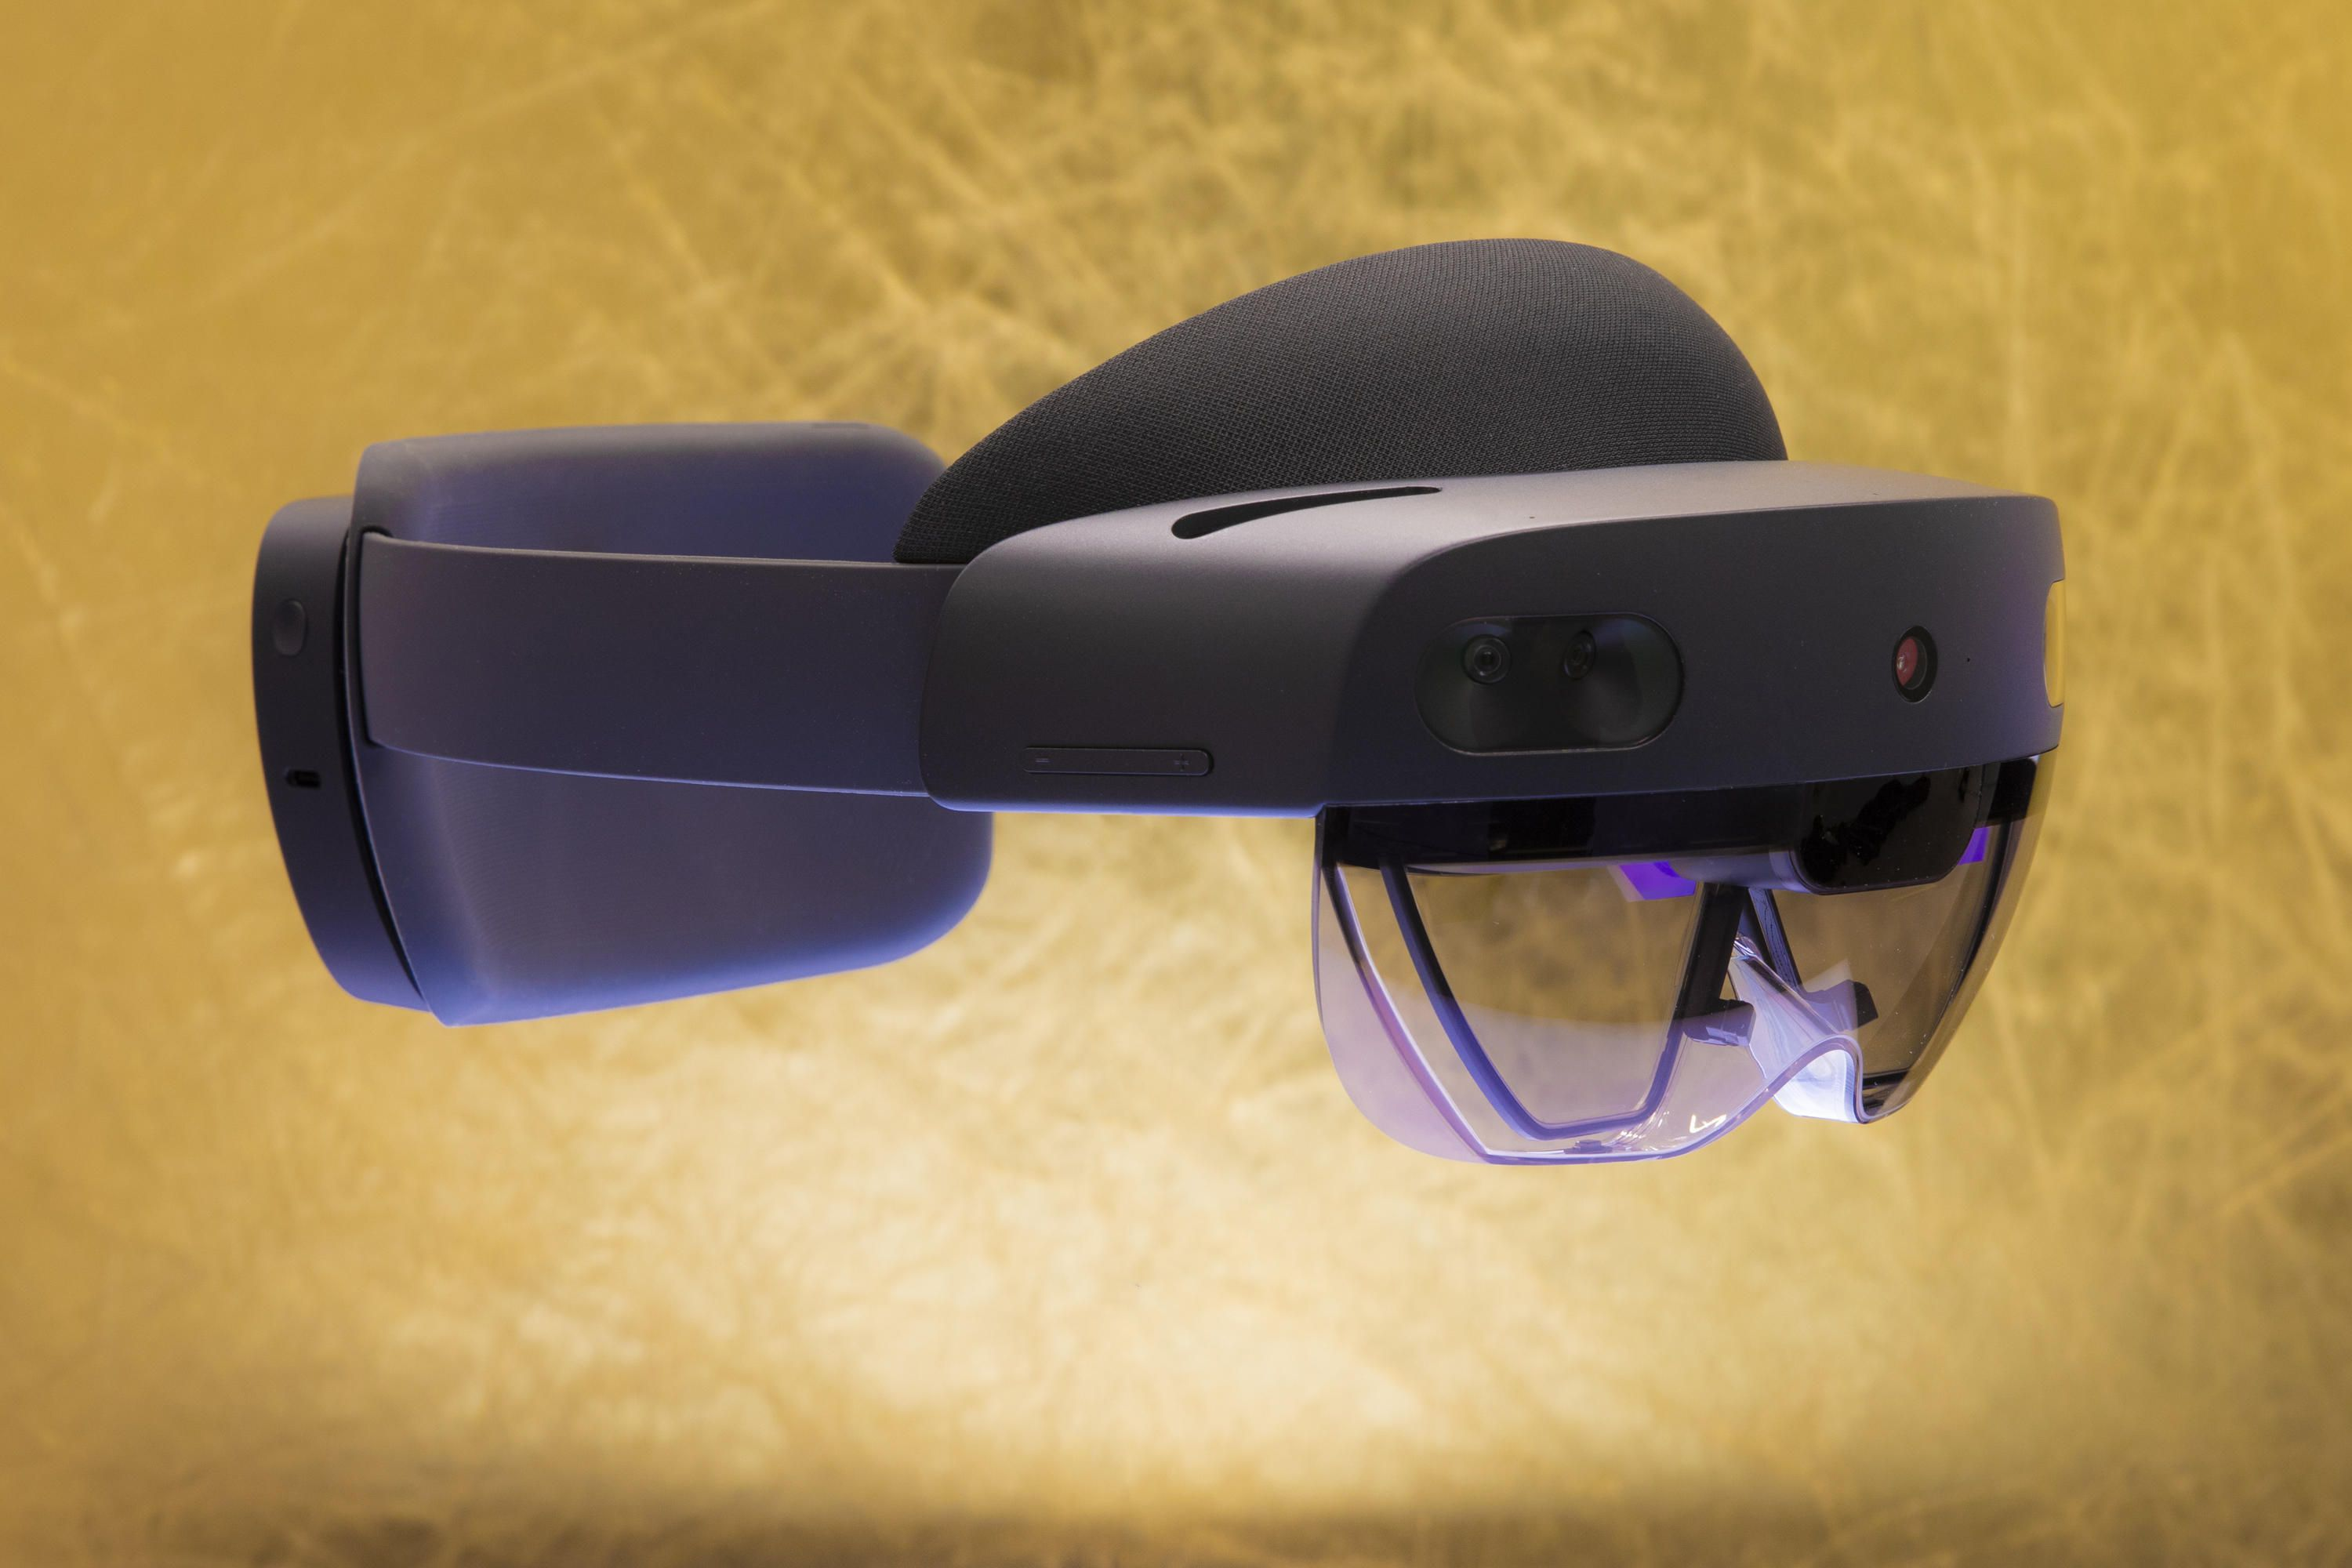
\includegraphics[scale=0.1]{images/holo.jpg}
	\caption{Hololens 2 kiterjesztett valóság szemüveg (forrás: \url{https://media.icdn.hu})}
	\label{fig:hololens}
\end{figure}

Az említett headset-ek kereskedelmi forgalomban kaphatók, ám magas áruk miatt nehezen terjednek. 

\SubSection{VR hardverek}

A virtuális tér kialakításához szükség van megfelelő hardverekre, mint például hangrenszer, kijelző (VR szemüveg), számítógép, telefon, konzol továbbá speciális szenzorok, amelyek követik a felhasználó mozgását (test, kéz, fej).

A következőket tekinthetjük a dolgozat megírásának idejében a leginkább elterjedt VR eszközöknek.
\begin{itemize}
\item {\bf Valve Index}: Remekül működik régebbi GPU esetén is, éles kijelzővel rendelkezik és a Valve kontroller képes az összes ujj mozgását követni. Azonban nehéz kalibrálni és beállítani. A magasabb árkategóriába tartozik.
\item {\bf Oculus Quest 2}: Könnyű a használata, azonban Facebook fiók hozzáadást igényel. \Aref{fig:occulus}. ábrán láthatunk róla egy képet.
\item {\bf PlayStation VR}: PS4 konzol szükséges hozzá. Sok játék elérhető hozzá. Nem a legjobbb a mozgás követésének a tekintetében.
\item {\bf Oculus Rift S}: Nem vezeték nélküli, így korlátoltabb a mozgás tér.  Kényelmesebb, mint az előző verziója, mivel könnyű. Viszonylag sok játék érhető el hozzá.
\item {\bf Samsung Gear VR}: Samsung okostelefonnal használható (Galaxy S8-tól felfelé).
\end{itemize}

\begin{figure}[htp]
    \centering
   	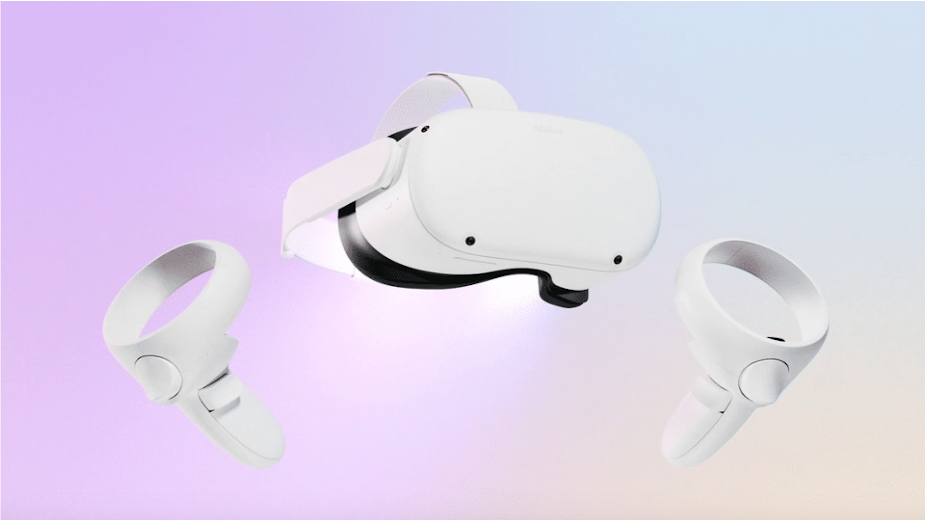
\includegraphics[scale=1]{images/oculus.png}
	\caption{Oculus Quest 2 virtuális valóság szemüveg és a hozzá tartozó vezérlők (forrás: \url{https://d3bzyjrsc4233l.cloudfront.net})}
	\label{fig:occulus}
\end{figure}

A következőkben néhány népszerű VR kontroller kerül említésre.
\begin{itemize}
\item \textbf{HTC Vive}: Képes követni a kéz mozdulatot, az ujjak mozgását.
\item \textbf{3DRudder}: Lábbal vezérelhető.
\item \textbf{SteelSeries Stratus XL}: Konzolhoz való kontroller kialakítású.
\end{itemize}

A VR kesztyűk egy külön alkategóriát képviselnek.
Precízebben lehet velük követni a kéz mozgását, külön követik a ujjak mozgását.
Ilyenek például az \textit{ExoGlove}, \textit{ManusVR} és a \textit{GloveOne} (\ref{fig:gloveone}. ábra).

\begin{figure}[htp]
    \centering
   	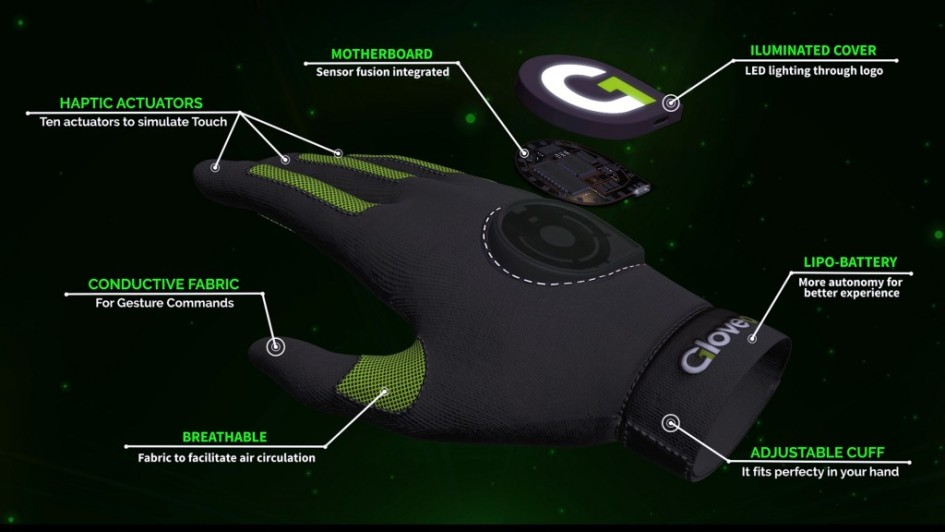
\includegraphics[scale=0.6]{images/gloveone.jpg}
	\caption{OneGlove VR kesztyű (forrás: \url{https://transhumanity.net})}
	\label{fig:gloveone}
\end{figure}

Érdekességképpen érdemes még megemlíteni a VR ruhákat, amelyek megpróbálják a lehető legközelebb hozni a felhasználót a virtuális térben lévő elemekhez.
Ilyen eszközök például a \textit{TeslaSuit} (\ref{fig:teslasuit}. ábra)) és a \textit{TactSuit}.

\begin{figure}[htp]
    \centering
   	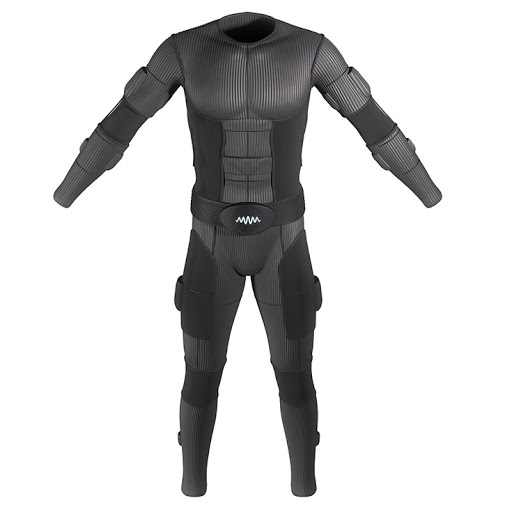
\includegraphics[scale=0.3]{images/tesla.jpg}
	\caption{TeslaSuit VR ruha (forrás: \url{https://uncrate.com/teslasuit})}
	\label{fig:teslasuit}
\end{figure}

\Section{A kiterjesztett valóság fajtái}

\SubSection{Marker alapú megoldások}

A markerek speciális azonosítók, amelyeket kamera segítségével, az AR alkalmazással felismerünk és a virtuális tartalmat (ami lehet egy  3D objektum például), a kamerához vizsonyított relatív pozicióba helyezzük el. 

Fontos, hogy a marker egyedi legyen és jól felismerhető a környezetben. 

Hátránya, hogy ha a marker egy része nem látható (például annak hatására, ha az eszköz elmozdul) akkor a tartalom eltűnik.
Marker lehet egyszerűbb információt hordozó bináris minta kerettel (például QR-kód vagy ArUco marker), síkbeli vagy térbeli objektum is.

\SubSection{Marker nélküli megoldások}

A marker nélküli kiterjesztett valóság jellemzően SLAM-et (\textit{Simultaneous Localization and Mapping}) használ környezet felmérése és követésére \cite{stachniss2016simultaneous}.
Érzékelheti például, hogy hol a padló, a plafon vagy a falak.
A megjelenített tartalmakat így a környezethez lehet viszonyítani, tájolni.

Lényeges elönye, hogy a virtuális tartalom itt nem tűnik el elmozdulás miatt, hisz nem egy adott markerhez,
hanem az egész környezethez számítja az alkalmazás annak pozícióját.

\Section{Szoftverek, fejlesztőeszközök}

A következőkben az elterjedt szoftveres eszközkészletek bemutatására kerül majd sor \cite{hanafi2019comparative}.

\SubSection{Apple ARKit}

Az Apple ARKit az iOS operációs rendszerrel (iOS 11-től felfelé) rendelkező eszközökre (iPhone, iPad amiknek minimum A9-es processzora van) való AR alkalmazások fejlesztéséhez használható. 
Például képes: 
\begin{itemize}
\item 2D-s kép felismerésére és annak követésére,
\item 3D-s objektum felismerésére és annak elhelyezésére a térben.
\item Az újabb verziókkal többjátékos módot támogató játékok készíthetők. 
\end{itemize}

\SubSection{Google ARCore}

A \textit{Google ARCore} igen népszerű AR SDK. Használható tabletre, telefonra való iOS és Android alkalmazások készítéséhez. Az SDK alapját a pozició követés és az objektum felismerés jelenti.
Fontos elemei az alábbiak.
\begin{itemize}
\item A fény követés a valósághűbb objektumok megjelenítéséhez.
\item Mozgás követés a telefon poziciójának felhasználásával.
\item Felismerése a felületek abszolút méretének, elhelyezkedésének függőlegesen és vízszintesen.
\end{itemize}

\SubSection{Vuforia}

A \textit{Vuforia} az egyik legnépszerűbb SDK a AR alkalmazások készítéséhez.

Annak köszönhetően, hogy \textit{Unity}-ben jól használható, lehetővé válik vele a Android-ra és iOS-re való natív alkamazások készítése (számos programozási nyelvet használva).

Asztali gépekre is lehet vele fejleszteni, szintén a Unity-nek köszönhetően. 
  
A következők a jellegzetes funkciói.
\begin{itemize}
\item  Kép, (angol nyelvű) szöveg, 3D-s objektumok felismerése és követése valós időben.
\item  Virtuális elemek elhelyezése a térben.  
\item  Virtuális gombok.
\item  Lokalizált okklúzió felismerés a virtuális gombok használatával.
\end{itemize}
Használható számos marker típussal, marker nélkül, markerként használt objektumokkal, \textit{VuMark}-kal (amely a QR-kód és kép együttese).

\SubSection{Wikitude}

A \textit{Wikitude} kíválóan alkalmazható hely-központú( WIFI vagy GPS felhasználásával) alkalmazások fejlesztésére telefonra. 

Népszerű az ipari felhasználás területén, annak köszönhetően, hogy a legrövidebb idő alatt ezzel lehet elkészíteni a vásárló-központú alkalmazásokat. 

Fő funkciói az alábbiak:
\begin{itemize}
\item 3D, kép felismerés és követés,
\item helymeghatározáson alapuló AR,
\item okos szemüveg integráció.
\end{itemize}

\SubSection{Kudan}

A \textit{Kudan} egy réteget add hozzá az objektumokhoz a felismerés megkönnyítése végett. Gyors és egészen egyszerű a használata. 
Használható markerrel és marker nélkül is.

\SubSection{ARToolKit}

Az \textit{ARToolKit} nyílt forráskodú (elérhető GitHub-on). Használható akár okosszemüvegekhez készített alkalmazások fejlesztéséhez is. Fejleszhető vele iOS, Android, Windows, MacOS és Linux platformra is alkalmazás. 
Rendelkezik \textit{Unity} és \textit{OpenSceneGraph} támogatással.
Megvalósítja az egy vagy duálkamerával való követést. Számos programozási nyelvvel használható.

\SubSection{EasyAR}

Az \textit{EasyAr} ingyenes, kiváló szoftveres eszköz kezdőknek. Van professzionális verziója is üzleti használatra, amely extra funkciókat tartalmaz. Androidra, iOS-re és Windows-ra van lehetőség fejleszteni vele.

\SubSection{MaxST}

A \textit{MaxST} két SDK-ra válik szét: egy a 2D kép felismeréshez, és egy a 3D objektumokhoz.
Felismeri a függőleges és vízszintes síkokat, így akár több objektumot is képes egyszerre követni. Alkalmas QR-kód és vonalkód szkenneléshez.

\SubSection{Pikkart AR SDK}

A \textit{Pikkart} SDK segítségével egyedi, funkció gazdag, felhasználóbarát alkallmazásokat lehet készíteni. Könnyű fejlesztési folyamatot biztosít.

\SubSection{AR.js}

Az \textit{AR.js} egy JavaScript alapú, nyíltforráskodú AR SDK. Böngészőben használható AR alkalmazások készítéséhez. Nem igényel semmilyen telepítést. Minden mobil platformon képes futni az ezzel az SDK-val készített alkalmazás.

\SubSection{További API-k}

Számos további API is elérhető. Név szerint említés szintjén például a következők:
\begin{itemize}
\item ARLab,
Onirix,
DeepAR,
MixedReality Toolkit (Hololens),
Xzimg,
DroidAR,
HP Reveal Studio,
BlippBuilder.
\end{itemize}

\Section{Unity}

A \textit{Unity} egy  olyan keresztplatformos játékmotor, amellyel lehetőségünk van Windows-ra, Linux-ra, Mac OS-re, iOS-re, Android-ra, valamint Wii-re és más játék konzolokra fejleszteni.

Van üzleti és személyi változata is. Bizonyos keretek alatt ingyenes lehet a cégeknek is, nem csak a magánszemélyeknek.

A hozzáférhető leírások alapján először a \textit{Unity} keretrendszer tünt megfelelőnek a dolgozatban bemutatott program elkészítéséhez.
A későbbiekben azonban számos probléma lépett fel, mint például a következők.
\begin{itemize}
	\item Túlságosan erőforrás igényes, speciális eszközöket igényelnek a kipróbálható demók (pl. VR szemüveg).
	\item A különböző verziókhoz tartozó leírásokban nehéz kiigazodni. Az adott problémákhoz fellelhető megoldások csak az adott verzión működtek.
\end{itemize}

\Section{Alacsonyabb szintű eszközök integrációja}

A korábban bemutatott, igen változatos és funkciókban gazdag eszközkészlet számos problémát hordozott magában.
Ezen okok miatt a fejlesztést egyszerűbb, de stabilan működő függvénykönyvtárak integrációjával tünt célszerűnek megoldani.
\begin{itemize}
	\item \textit{OpenCV}: Gépi látáshoz használt függvénykönyvtár.
	\item \textit{OpenGL}: Nyílt grafikus nyelv és a hozzá tartozó függvénykönyvtár.
\end{itemize}
A Python programozási nyelv alkalmasnak bizonyult arra, hogy ezek funkcióihoz egyszerűen hozzá lehessen férni, azokat egy alkalmazásba könnyen lehessen integrálni.

\Chapter{Kamerapozíció becslése a virtuális térben}

Ahhoz, hogy a virtuális tér elemeit a valós térből kapott képre rá lehessen illeszteni, meg kell tudni becsülni, hogy a kamera abban hol helyezkedik el.
Erre többféle lehetőség is adódik.
A fejezetben ezek áttekintésére kerül sor.

\Section{Markerek}

A markerek olyan, fizikális jelölő pontok, amelyeket képfeldolgozási módszerekkel, a\-rány\-lag nagy megbízhatósággal be lehet határolni a kameraképen.
Az AR/VR technológiák fejlődésével az egyszerűbb, szembetűnő markerektől fokozatosan jutott el a technológia a betanítható markerekig (illetve a marker nélküli megoldásokig).
A következő szakaszokban a két jellegzetes megközelítés kerül részletezésre.

\SubSection{Klasszikus markeres megoldások}

A kiterjeszetett valóság fontos eszköze a markerek, így azok használata jól támogatottnak mondható. Számos nyílt forráskodú könytár rendelkezésre áll a klasszikus értelemben vett markerekből.

\bigskip

\noindent \textbf{Vonalkód, QR-kód}

\medskip

A vonalkódokat és a QR kódokat az információ tároláson túl használhatjuk pozíció becslésére is.
A QR-kód neve \textit{Quick Response}-t, vagyis gyors választ jelent.
Ez egy kétdimenziós kód. Működésében nagyon hasonlít a vonalkódhoz, gyakorlatilag annak egy fejlettebb változatáról van szó.
Míg egy vonalkód esetében jellemzően 13 számjegy kerül tárolásra, addig a QR kód akár 7000 számjegyet és 4300 alfanumerikus karaktert tud kódolni. (Tipikusan például egy weboldal URL-jét.)
Ezekre láthatunk egy-egy példát \aref{fig:barcode}. ábrán.

\begin{figure}[htp]
    \centering
   	
\includegraphics[scale=0.25]{images/qr_bar.png}
	\caption{Példa vonalkódra és QR-kódra}
	\label{fig:barcode}
\end{figure}

\bigskip

\noindent \textbf{„Keretes” markerek}

\medskip

Az ilyen típusú markerek két részből állnak; egy fekete keretből, ami a felismerést segití és egy belső mintából. A belső minta lehet kép, egyedi bináris minta, amely azonosítja a markert, információt hordoz.

A keret fontos szerepet tölt be, hisz egy fekete téglalapot/négyzetet viszonylag egyszerűen és gyorsan fel lehet ismerni egy képen, meghatározni annak pozícióját a kamerához képest, sarok pontjait, a középpontját.

Ilyen típusú marker például az \textit{ARToolKit} marker (amelynél középen egy kép van, ami bináris képként lesz kezelve), \textit{ARTag}, \textit{AprilTag} és az \textit{ArUco}.

Kombinálni is szokták az egyszerűbb markereket: a QR-kódot és a kerettel rendelkező markereket, vagy a QR kód van a keret belsejében vagy pedig a QR kód közepén szerepel például egy ArUco marker vagy egy kép (mint például a \textit{VuMark} esetén).
Ezekre láthatunk példákat \aref{fig:markerek}. ábrán.

\begin{figure}[htp]
    \centering
   	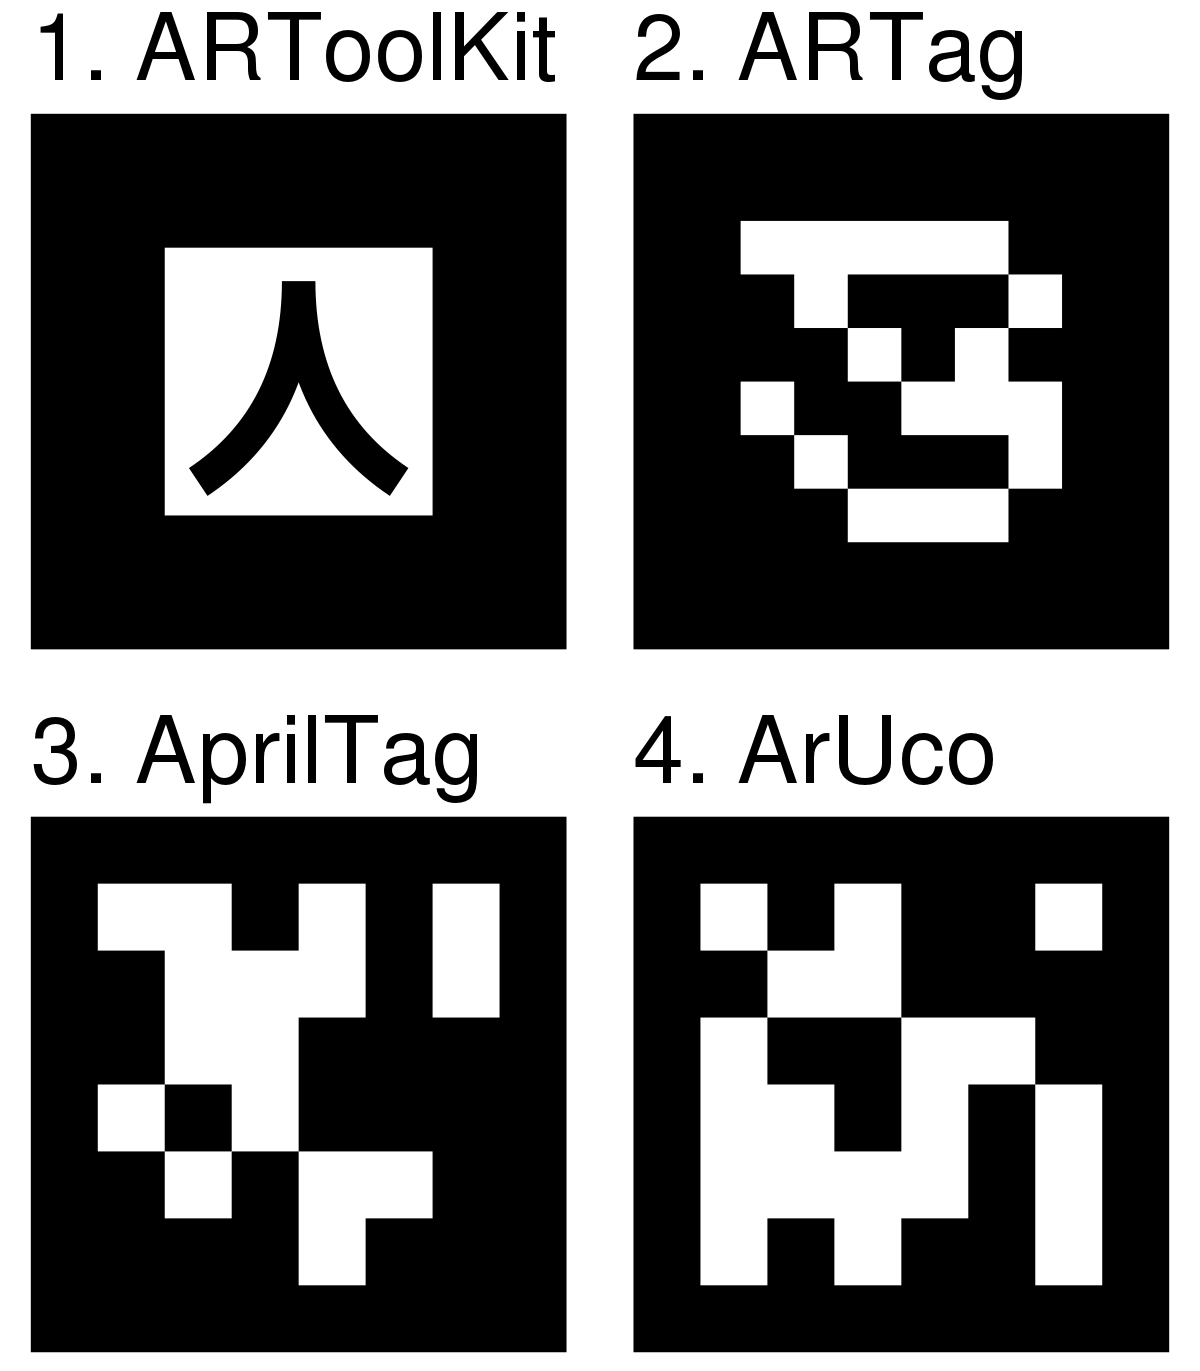
\includegraphics[scale=0.25]{images/markerek.png}
	\caption{ArToolKit, ARTag, AprilTag, ArUco}
	\label{fig:markerek}
\end{figure}

\SubSection{Betanítható markerek}

A kiterjesztett valóság technikai fejlődéssel a markerek is bonyolultabbá váltak, lehetőség nyílt hétköznapi tárgyak, épületek és egyéb valós objektumok markerként történő kezelésére.

Természetesen ezek detektálása nehezebb, illetve betanítást igényel.

Léteznek továbbá úgynevezett marker nélküli (\textit{markerless}) AR alkalmazások is, amelyekben a szenzorok felmérik környezetet és megfelelő helyre pozicionálják a megjelenítendő objektumot/objektumokat. Egy ismert példa erre a földrajzi koordináták felhasználásával működő \textit{Pokemon GO} játék.

\Section{Inerciális szenzorok}

A fejlettebb telefonokban található inerciális szenzorok fontosak a kiterjeszett valóság felhasználásával készült alkalmazások müködtetéséhez.

Az inerciális szenzorok gyorsulásérzékelőkből és giroszkópokból állnak, minél nagyobb a számuk, annál pontosabb eredményeket képesek biztosítani.

Az inerciális szenzorokkkal a telefon térbeli helyzetének és annak változára vonatkozó adatokat kaphatunk meg.

Az accelerométer a telefon helyzetének változását méri a $x$, $y$ és $z$ tengelyeket alapul véve.

A telefonokban található giroszkóp (vagy röviden \textit{gyro} szenzor) a gyorsulásmérő egy fejlettebb verziója.
Míg accelerometer tengely alapú elmozdulást mér, addig a giroszkóp az acceletométert felhasználva minden apró változást érzékel. Pontosabb adatokat kaphatunk vele.
\Aref{fig:inertial}. ábrán láthatjuk, hogy például hogyan néz ki egy ilyen szenzor.

\begin{figure}[htp]
    \centering
   	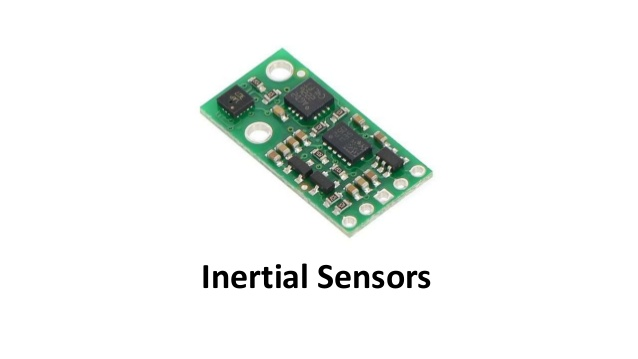
\includegraphics[scale=3]{images/inertial.jpg}
	\caption{inerciális szenzor}
	\label{fig:inertial}
\end{figure}

\Section{Az Aruco marker használata}

Az \textit{ArUco} (\textit{Augmented Reality University of Cordoba}) markereket 2014-ben fejlesztette ki kollégáival S. Garrido-Jurado Spanyolországban.
Az ArUco könyvtár OpenCV alapú, nyílt forráskódú, C++ nyelvű függvénykönyvtár.
Ar ArUco markerek két részből állnak: egy fekete keretből és az egyedi bináris mintából, ami azonosítja a markert (mint ahogy például \aref{fig:kep}. ábrán látható).

Alapvetően az OpenCV-s támogatottsága miatt került kiválasztásra a dolgozatban felvetett kamerapozíció becslési problémákhoz. A detektálást számos beépített függvény segíti.

\begin{figure}[htp]
    \centering
   	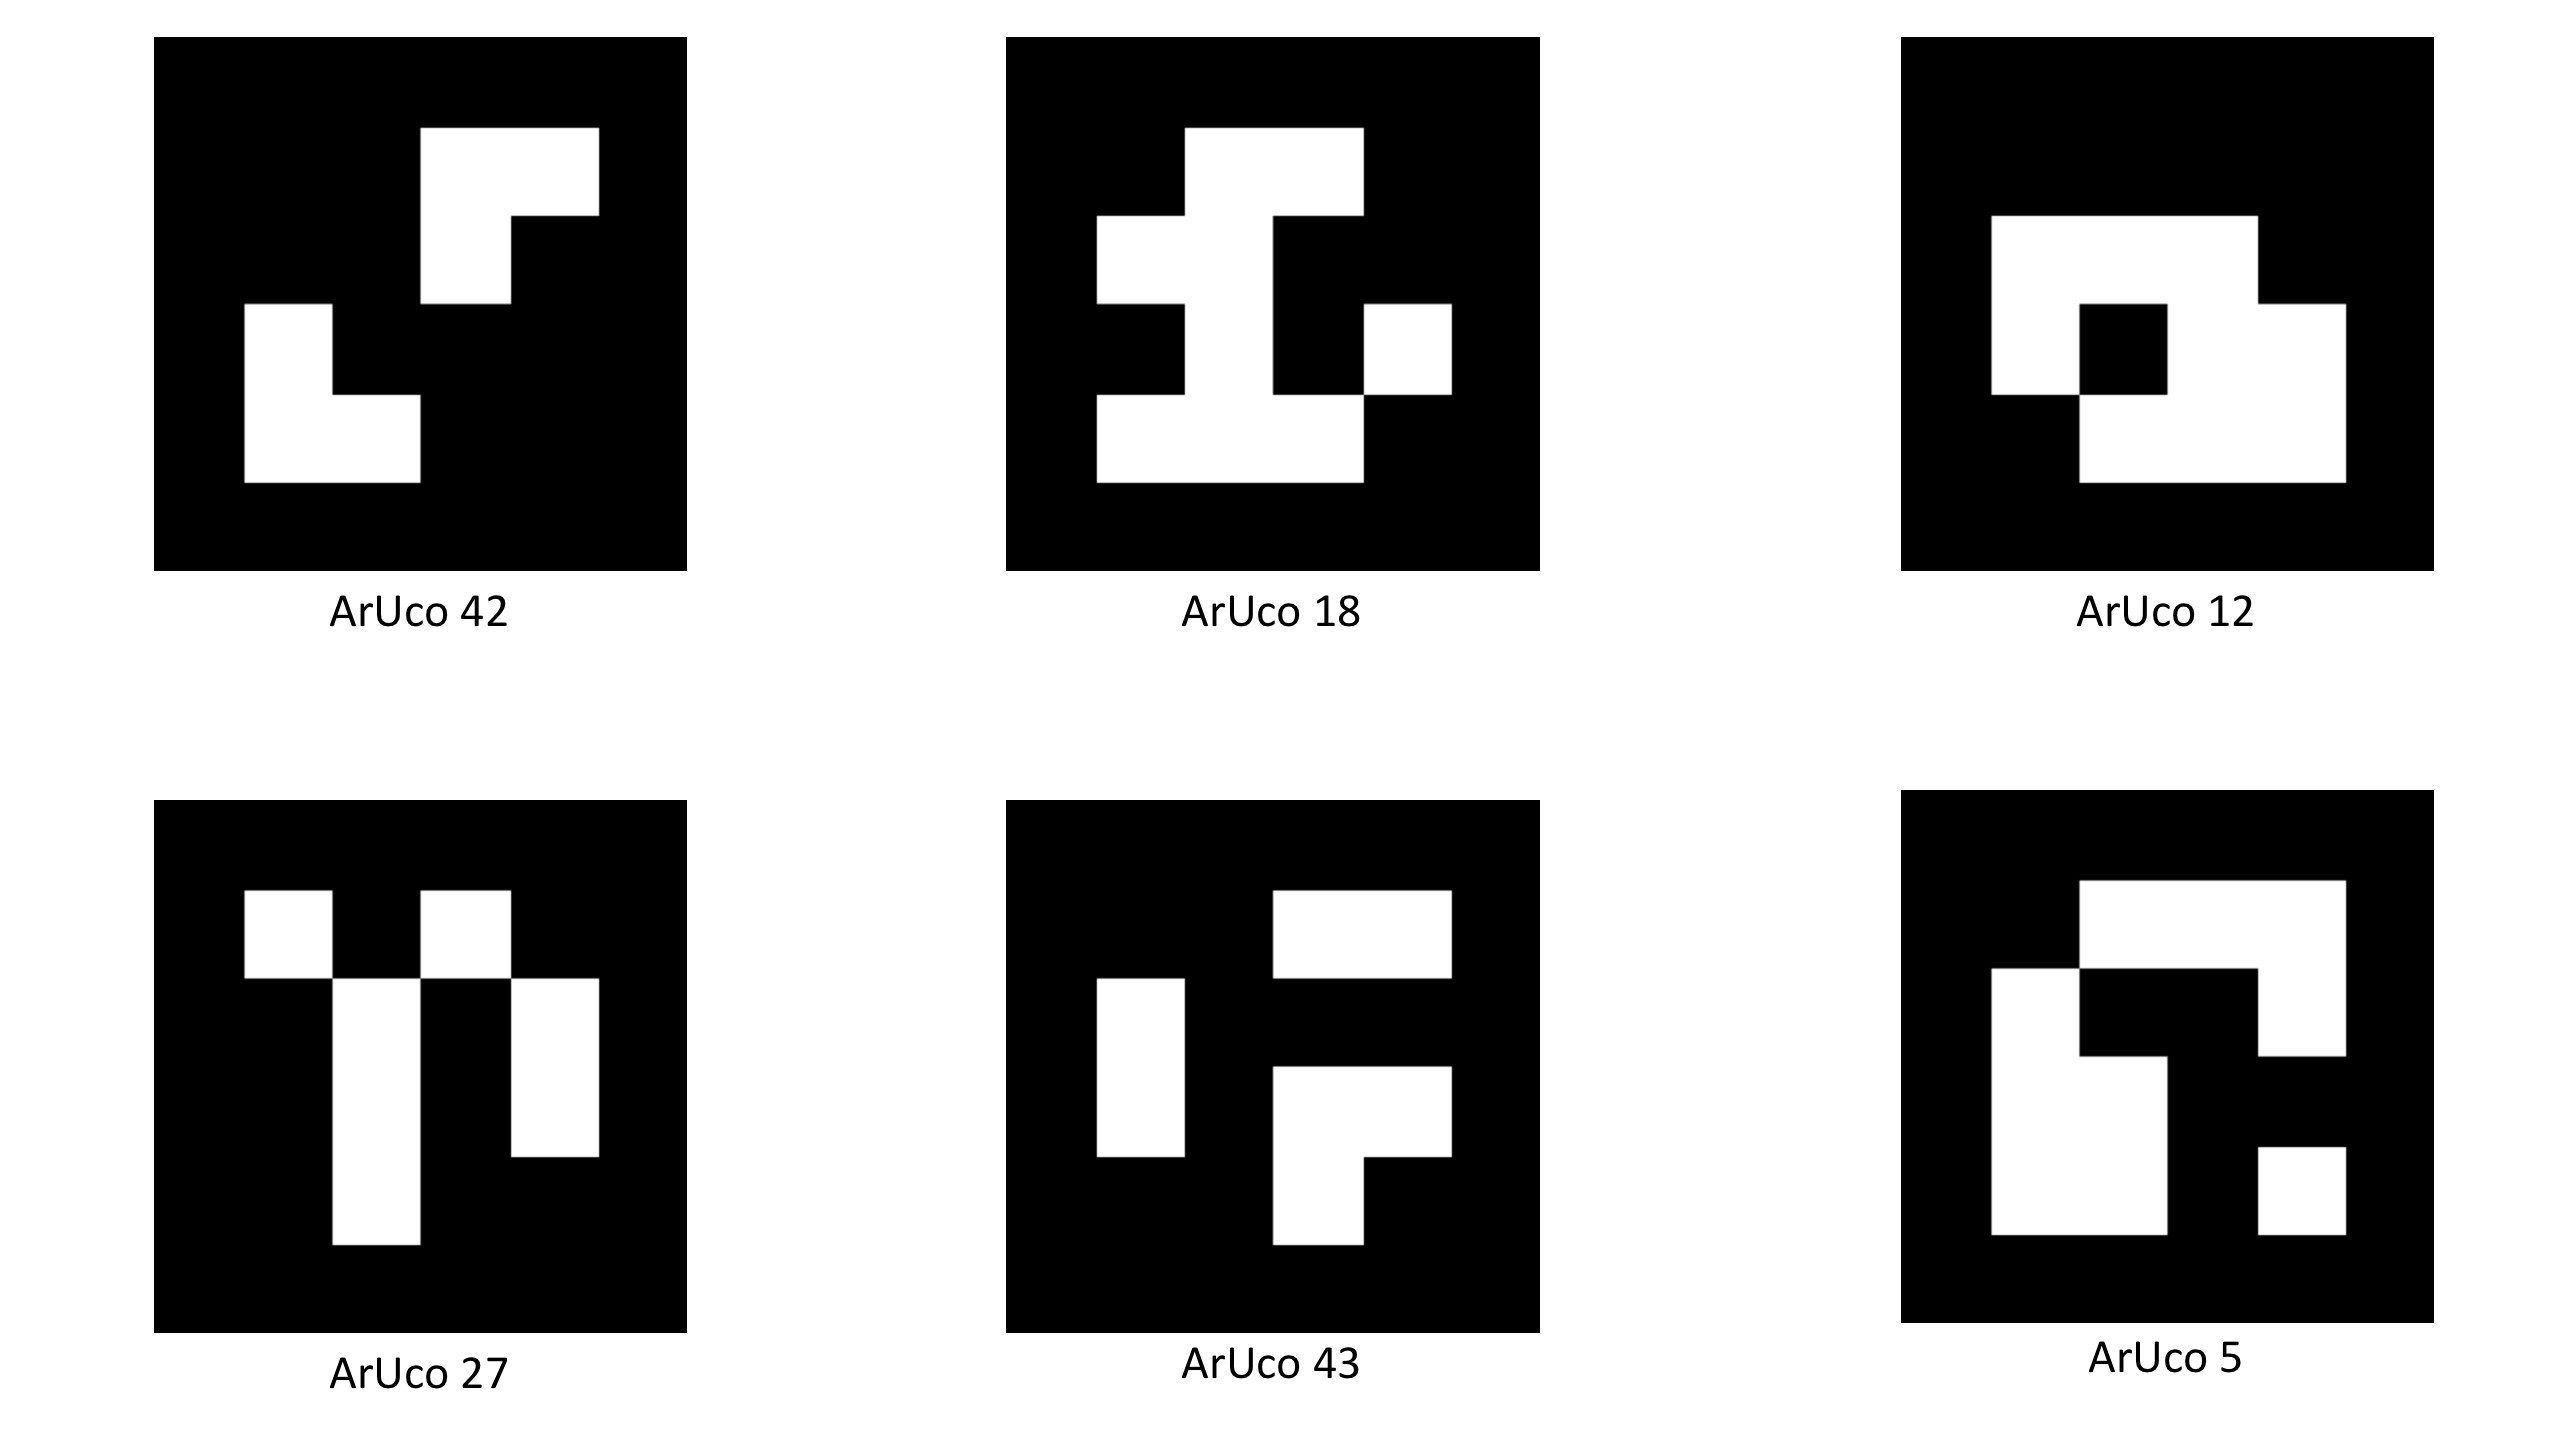
\includegraphics[scale=0.4]{images/kep.png}
	\caption{Aruco markerek a $4 \times 4$-es könyvtárból}
	\label{fig:kep}
\end{figure}

\SubSection{Típusai, használati módok}

Az ArUco markerekhez különböző könyvtárak érhetőek el, amelyek a marker méretében (szükséges bitek száma), belső minta oszlop és sor számában (az oszlop és sor szám mindig megegyezik) és az elérhető azonosítók számában térnek el.
A bináris minta $4 \times 4$-től a $7 \times 7$ bitig terjed (amelybe nem számít bele a keret).

Minél bonyolultabb egy minta, és minél nagyobb annál nehezen felismerni, ezért a \texttt{DICT\_4X4\_100} használata tünt megfelelő választásnak.

Ennél a \texttt{\_4x4} a bitek számát, a \texttt{100} pedig a könyvtárban lévő markerek azonosítóit jelöli.
Ez azt jelenti, hogy az azonosítók 0 és 99 között vannak.

\SubSection{Kamera kalibrálása}

% TODO: https://medium.com/@aliyasineser/aruco-marker-tracking-with-opencv-8cb844c26628

A kamera kalibrációjához $6 \times 9$-es sakktábla mintát használtam (\ref{fig:calibration}. ábra). (A külső sáv nem számolandó bele, az a felismerést könnyíti, a belső minta számít.)

\begin{figure}[htp]
	\centering
	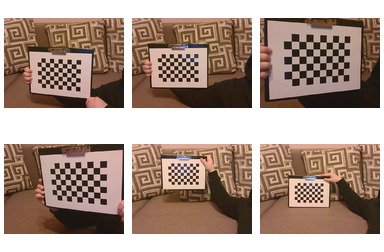
\includegraphics[scale=1]{images/calibration.jpg}
	\caption{Kalibráláshoz használt képek közül néhány}
	\label{fig:calibration}
\end{figure}

A kalibráció eredményességéhez a négyzeteknek szabályosnak, egyformának kell lenniük és fontos, hogy a nyomtatás során a minta ne torzuljon el, ne legyen átméretezve.

A pontosság növelése érdekében a képeket érdemes minél változatosabb szögben és távolságból elkészíteni. Valamint ügyelni kell arra, hogy a lap egyenes legyen tartva, ezért célszerű megfelelő támaszt használni hozzá.

A kalibráció során kapjuk meg a későbbiekben nélkülözhetetlen együttható (kamera) mátrixot, a disztorziós együtthatókat, az eltolási és forgatási vektorokat.

A kalibrációt végző függvénynek a sorok és oszlopok számára, a négyzetek oldalhosszára és a fent említett képekre van szüksége.

A folyamat során meg kell határozni a fekete-fehérré tett képen szereplő a sakktábla minta sarokpontjait
\texttt{findChessboardCorners()} függvénnyel, majd pontosabbá tenni azok koordinátáit
\texttt{cornerSubPix()}-lel, például az alábbi módon.
\begin{python}
ret, corners = cv2.findChessboardCorners(gray, (width, height), None)
...
corners2 = cv2.cornerSubPix(gray, corners, (11, 11), (-1, -1), criteria)
\end{python}
Az ezzel kapott pontokat (projekciós pontjai a sakktáblába mintának) az objektum pontjait (a minta pontjai a minta terében), továbbá a kép méretét kell megadni a \texttt{calibrateCamera()} függvénynek.
\begin{python}
ret, mtx, dist, rvecs, tvecs = cv2.calibrateCamera(objpoints,
  imgpoints, gray.shape[::-1], None, None)
\end{python}
Ez ebből kapott értékek a következők:
\begin{itemize}
\item {\bf cameraMatrix}: $3 \times 3$ lebegőpontos kamera mátrix
\[
A =
\begin{bmatrix}
	f_x & 0 & 0 \\
	0 & f_y & 0 \\
	0 & 0 & f_z \\
\end{bmatrix}
\]

\item {\bf distortionCoefficient}: Bemeneti/kimenti torzítási együttható vektor:
\[
(k_1, k_2, p_1, p_2, [, k_3 [, k_4, k_5, k_6, [, s_1, s_2, s_3, s_4 [, \tau_x, \tau_y]]]])
\]
amely 4, 5, 8, 12 vagy 14 elemből állhat.

\item {\bf rvecs}: A mintákhoz tartozó elforgatási vektorok becsült kimeneti vektora.

\item {\bf tvecs}: A mintákhoz tartozó vektorok becsült kimeneti vektor
\end{itemize}

\SubSection{Demo alkalmazás}

A markerek detektálásának eredményességét befolyásolják a fényviszonyok, a kamerához viszonyított pozíció, a minta bonyolultsága, a szög amiben látszik és a mérete. Továbbá óriási hátrány, hogy ha takarásba kerül egy része a markernek (legyen ez akármilyen kicsi), mivel akkor nem lesz felismerhető.

Az ArUco marker felismerésére használt demó alkalmazás bekalibrálja a kamerát (ha ez még nem történt meg), majd a kalibrációból kapott \texttt{camera\_matrix} és a \texttt{dist\_Coefficient} felhasználásával detektálja a markert az élő képen.

A folyamatos kapcsolat érdekében egy végtelen ciklus van a programban.
Ezután kapcsolatot kell teremteni a kamerával és mindig az adott pillanatnyi képpel dolgozni.
Ehhez az OpenCV \texttt{VideoCapture} függvényére van szükség. A 0 index a laptop saját beépített kameráját jelöli, ha csatlakoztatható USB-s kamerával szeretnénk dolgozni, akkor az 1 paramétert kell megadni.
\begin{python}
cap = cv2.VideoCapture(0)
...
ret, frame = cap.read()
\end{python}
A kamera kép olvasásakor visszakapott második paraméterre lesz szükségünk, ami maga a kép. Ha valamilyen okból kifolyólag nem sikerül olvasni, akkor hamis értékkel és üres képpel tér vissza.

Ha meg van a kép, meg kell adni a megfelelő könyvtárat, amiben szerepel a marker, amit fel akarunk ismerni. Jelen esetben ez a \texttt{DICT\_4X4\_100}.
\begin{python}
aruco_dict = aruco.Dictionary_get(aruco.DICT_4X4_100)
\end{python}
Ezt a változót, a paramétereket, a képet, a kamera mátrixot és disztorziós együtthatókat felhasználva detektáljuk a markert a \texttt{aruco.detectMarker()} függvény segítségével.
\begin{python}
corners, ids, rejectedImgPoints = aruco.detectMarkers(image, aruco_dict,
parameters=parameters,
cameraMatrix=mtx,
distCoeff=dist)
\end{python}
Eredményként a megtalált markerek sarokpontjait és a belső minta által definiált azonosítókat kapjuk vissza.

A sarokpontokat és a kamera mátrixot és a disztorziós együtthatót felhasználva a
\texttt{estimatePoseSingleMarkers} meghatározza a marker elfordulását és eltolását a kamerához képest.

Ezután  mindenezt felhasználva a képen talált markert a program  körbe rajzolja, kijelöli a felső sarok pontját és ráteszi a képre a marker koordináta rendszeréhez tartozó triédert.
\begin{python}
rvec, tvec ,_ = aruco.estimatePoseSingleMarkers(corners,
0.17, matrix_coefficients, distortion_coefficients)
aruco.drawAxis(frame, matrix_coefficients, distortion_coefficients,
rvec, tvec, 0.01)
\end{python}
Erről láthatunk egy képet \aref{fig:felismeres_aruco}. ábrán.
\begin{figure}[htp]
    \centering
   	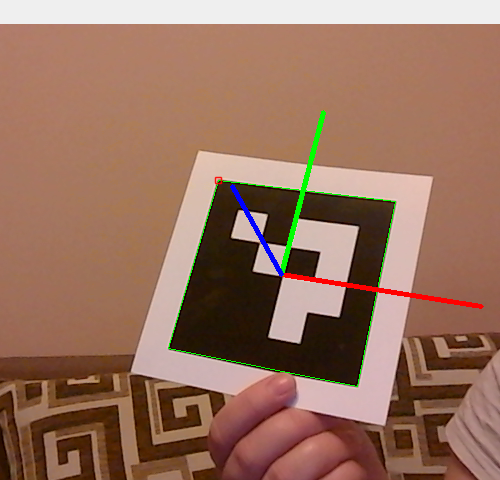
\includegraphics[scale=0.6]{images/felismeres_aruco.png}
	\caption{A demó eredménye}
	\label{fig:felismeres_aruco}
\end{figure}

\SubSection{A marker felismerésére készített program tesztje}

A végső programban az ArUco marker felismerés egy olyan függvényként jelenik meg, ami megkap egy képet és ha talál rajta markert, akkor visszaadja a megfelelő vektorokat (elforgatás és eltolás vektorokkal).

Ezen programrésznek a tesztelésére készítettem a nyomtatott markeremről képeket, és megnéztem milyen eredményeket ad vissza és felismeri-e a képen szereplő markert.

Azon kijelentés, hogy ha takarásba kerül a marker bármely része, akkor nem lesz továbbá felismerhető teljesen helytálló, mivel a program nem találta meg a markert, hogy ha annak egy aránylag kis része már ki volt takarva.

A programban az eredményt a vektorokat a fent már említett \texttt{estimatePoseSingle} \texttt{Markers} adja vissza.

Az \texttt{rvec} a marker kamerához képest vett elfordulása az $x$, $y$ és $z$ tengelyeken, a \texttt{tvec} pedig a marker eltolása ugyanezekhez. Tehát egy markerhez két vektorhármast kapunk vissza.

Ezen vektorok fogják a későbbiekben meghatározni a kirajzolandó modellek helyét a térben.

A lentebb szereplő képekhez kapot értékek közül néhány:
\begin{itemize}
\item 1. kép \texttt{rvec} és \texttt{tvec} értékei::
\[[-0.00010618, -0.00181233, 0.04695004]\]
\[[ 1.91320312, -1.6522394,  0.60923043]\]
\item 2. kép \texttt{rvec} és \texttt{tvec} értékei::
\[[-0.00082155,  0.00022395,  0.06280824]\]
\[[ 1.83895896, -1.46640971,  0.69940467]\]
\item 3. kép \texttt{rvec} és \texttt{tvec} értékei:
\[[-0.00619668, 0.00013297,  0.04769506]\]
\[[ 1.87260078 -1.66750728  0.64313328]\]
\item 5. kép \texttt{rvec} és \texttt{tvec} értékei:
\[-0.00501719, -0.01433891,  0.08986719]\]
\[[ 1.25084371,  2.11521712, -1.07834937]\]
\end{itemize}

Látható például, hogy az 5. kép eltolási és forgatási vektorainak értéke nagyobb, mint a 1. vagy 2., hisz ez messzebb van a képen a kamerához képest és jobban el van forgatva, mint a másik kettő.
Természetesen ha nem ismeri fel a amerkert, vagy nincs marker a képen 0 értéket add vissza a program.

\Aref{fig:detect}. ábrán láthatunk olyan képeket, amelyeknél sikeres volt a marker detektálása, \aref{fig:not_detect}. ábrán pedig olyanokat, amelyre sikertelen.

\begin{figure}[htp]
    \centering
   	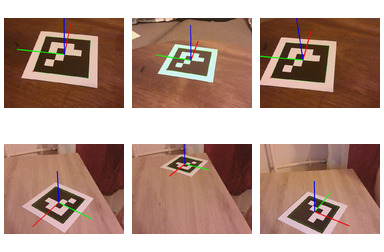
\includegraphics[width=\textwidth]{images/detect.jpg}
	\caption{Sikeres detektálás}
	\label{fig:detect}
\end{figure}

\begin{figure}[htp]
    \centering
   	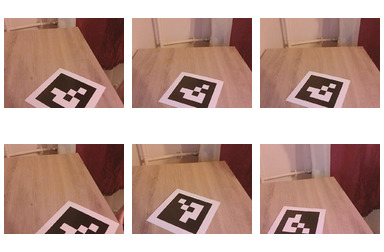
\includegraphics[width=\textwidth]{images/not_detect.jpg}
	\caption{Sikertelen detektálás}
	\label{fig:not_detect}
\end{figure}

\Chapter{A virtuális kollaborációs tér}

% A fejezet gyakorlatilag a kliens kialakításáról szól.

% Maga a menü, beállítások és egyéb felületi elemek is lehetnek 3D-sek.

A dolgozat elsődleges célja, hogy egy AR/VR alapú kollaborációs teret hozzon létre.
A fejezet ennek a megjelenítési módjával és a virtuális térben való interakciónak a leírásával foglalkozik.

\Section{Megjelenítési mód}

A megjelenítési mód OpenGL alapú.
A következő szakaszokban ennek a Python nyelvű implementációja kerül részletezésre.

\SubSection{OpenGL, PyOpenGL}

Az OpenGL egy grafikus nyelv, amely függvénykönyvtár formájában rendelkezésre álló implementációjával 2D-s és 3D-s alakzatokat tudunk megjeleníteni. Nagyon elterjedt, elérhető és támogatott a fő operációs rendszereken (Linux, macOS, Windows), valamint számos programozási nyelvvel kompatibilis \cite{opengl}.

Az OpenGL pythonnal használható verziója a cross-platform, nyíltforráskodú \textit{PyOpenGL}. A PyOpenGL támogatja a GL, GLU és GLUT könyvtárakat.
Továbbá lehetőség van a \textit{PyGame} függvénykönyvtár használatára OpenGL-s kódok megvalósításához.

A dolgozathoz tartozó program felhasználja mindhárom könyvtárat, és a modell betöltéshez a \textit{PyGame}-et is.

\SubSection{Modellek}

A program Wavefront OBJ formátumú modellekkel dolgozik, amelyekhez anyagjellemzőket leíró, \texttt{mtl} kiterjesztésű fájlokkal textúrát is rendelhetünk. 
\begin{itemize}
\item \texttt{obj}: A Wavefront Technologies által a Advanced Visualizer animációs csomagjukhoz kifejleszett obj fájlformátum egy geometria-definíciós formátum. 
Annak köszönhetően, hogy nyílt formátum, más 3D-s grafikus alkalmazások gyártói átvették.

Az obj egy egyszerű formátum ( akár ember által is olvasható), ami semmi mást nem add meg, mint a 3D geometriát, mint például a csúcsok helyzetét, az egyes textúra koordináta-csúcsok helyzetét, a csúcsok normálisát, az egyes sokszögeket csúcsok listájaként, textúra csúcsokat \cite{obj}.

\item \texttt{mtl}: Az MTL fájl egy segédfájl, amely a modell anyagainak meghatározását tartalmazza, amelyekhez OBJ fájl hozzáférhet. Az OBJ fájlnak meg kell adnia az MTL fájl nevét. Az MTL fájl az anyagok definícióinak sorrendjét tartalmazza. Mindegyik definíció egy newmtl utasítással kezdődik, amely meghatározza az anyag nevét, majd azon sorok következnek, amelyek megadják az adott tulajdonságokot \cite{mtl}.
\end{itemize} 

A program fő elemei az ágensek. 
A modell, amit felhasználtam erre a célra egy császárpingvin (\ref{fig:pingvin}. ábra). 
Minden ágenst ilyen modellel jelenít meg a program, csupán a színük változik, ami pedig a programkódban kerül megvalósításba.

\begin{figure}[htp]
    \centering
   	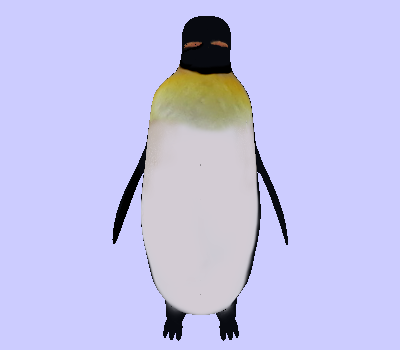
\includegraphics[scale=0.6]{images/pingvin.png}
	\caption{császárpingvin modell}
	\label{fig:pingvin}
\end{figure}

A program szinterének fő eleme a kastély modell, ahol maga a jelenet játszódik (\ref{fig:castle}. ábra).

\begin{figure}[htp]
    \centering
   	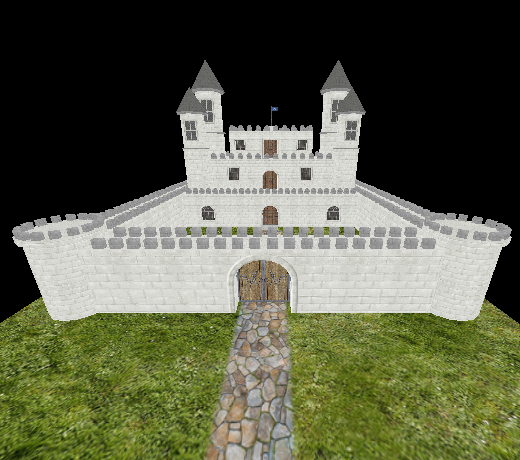
\includegraphics[scale=0.7]{images/castle.png}
	\caption{kastély modell}
	\label{fig:castle}
\end{figure}

Felhasználtam továbbá doboz modelleket, amiknek az elmozgatása a feladat (\ref{fig:box}. ábra). Ezen modellek színének manipulációja szintén a programban történik.

\begin{figure}[htp]
    \centering
   	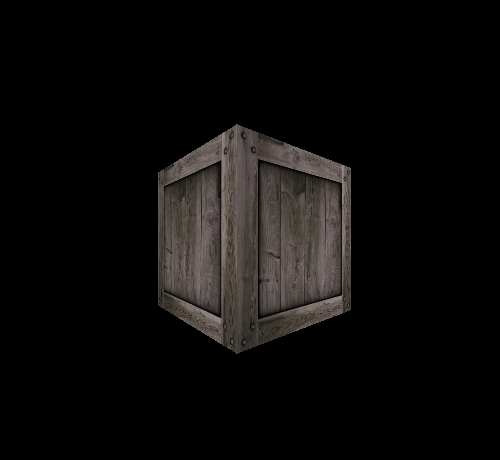
\includegraphics[scale=0.5]{images/box.png}
	\caption{doboz modell}
	\label{fig:box}
\end{figure}

%\SubSection{Fények és anyagjellemzők}
%
%Az objektumok megjelenítéséhez elengedhetetlenek a megfelelő fénybeállítások.
%A szokásos fényösszetevőket használhatjuk ez esetben is.
%
%\begin{itemize}
%\item A {\bf környezeti fény} (\texttt{ambient light}) az ábrázolandó térrészben mindenütt jelen lévő, állandó intenzitású fény, amelynek forrása, iránya nem ismert (gondoljunk olyan nappali fényre, amikor a nap a felhők mögött van).
%\item A {\bf szórt fénynek} (\texttt{diffuse light}) van iránya, mindig valamelyik fényforrásból jön. Fő jellemzője, hogy az objektumokkal ütközve minden irányba azonos módon és mértékben verődik vissza, tehát teljesen mindegy, hogy milyen irányból nézzük az objektumokat, a hatás csak a fényforrástól, az anyagtulajdonságoktól és a pontbeli normálistól függ.
%\item A {\bf tükröző fénynek} (\texttt{specular light}) is van iránya és forrása, és hatása nemcsak az anyag-tulajdonságoktól és a pontbeli normálistól, hanem a nézőponttól is függ. Gondoljunk egy sima felületű fémgömbre, amit erős, koncentrált fénnyel világítunk meg. Megfelelő szögből nézve egy fényes (többnyire fehér) foltot látunk, amelynek mérete és helye a nézőponttól függ, fejünket mozgatva a folt is mozog, mígnem eltűnik. \cite{fenyek_szinek}
%\end{itemize}
%
%\SubSection{A modellek átszínezése:}
%
%A modellek átszínezésére az OpenGL \texttt{glColorf} függvényét használtam, ahhoz azonban hogy ezt alkalmazni tudjuk, meg kell érteni, miként értelmezzük a színeket a számítógép grafikában.
%
%,,A színeket legcélszerűbb egy háromdimenziós tér pontjaiként felfogni. A tér egy bázisának(koordináta-rendszerének) rögzítése után minden színt egy számhármas segítségével lehetazonosítani. A számítógépi grafikában két színmegadási (színkeverési) mód, kétféle bázisterjedt el.”
%\begin{itemize}
%\item  RGB (additív): ,,Additív színkeverés esetén azt írjuk elő, hogy mennyi vörös (Red), zöld (Green) és kék (Blue) színkomponenst adjunk a fekete színhez, a fekete képernyőhöz.”
%\item CYM (szubtraktív): ,,Szubtraktív színkeverés esetén azt írjuk elő, hogy mennyi türkiz (Cyan), bíbor (Magenta) és sárga (Yellow) színt kell kivonnunk a legösszetettebb színből, a fehérből (a papírszíne) a kívánt szín előállítása érdekébe.”\cite{fenyek_szinek}
%\end{itemize}
%
%A \texttt{glColor} az RGB bázisrendszert használja fel, tehát a három paramétere egy-egy szám, ami a piros, zöld és kék színeket jelöli.
%
%A \texttt{glColor3*}, ahol a * a számok típusát jelöli.(int,float...) Az egész számokra vonatkozó változata a \texttt{glColor3i}), a float \texttt{glColor3f},továbbá a \texttt{glColor4*} rendelkezik egy negyedik paraméterrel is, az \texttt{alpha}-val, ami az átlátszóságot határozza meg.
%Például: 
%\begin{python}
%glColor3f(0.0,0.0,0.0) #fekete
%glColor3f(1.0,1.0,1.0) #feher
%glColor3f(1.0,0.0,0.0) #piros
%glColor3f(0.0,1.0,0.0) #zold
%glColor3f(0.0,0.0,1.0) #kek
%\end{python}

\Section{Interaktív elemek}

A színtér interkatív elmei az ágensek és a dobozok. 
Az ágensek képesek fordulni, előrehaladni, ugorni. 
A dobozok pedig olyan irányú elmozdulásra, amerre tolják őket.

\SubSection{Animáció}

Ahhoz, hogy a program látványosabb legyen animációkra van szükség, így a modell nem csak elmozul például olyan írányba, amerre szeretnénk, hanem az animáció használata séta hatását kelti.

A modellek formátuma azonban nem támogatja az animációkat, ezért minden egyes mozdulatnak külön modell készült (a hozzátartozó mtl fájllal).

Az animációk elkészítéséhez elsőnek a modell úgynevezett vázára van szükség, azt kell elkészíteni, és azt lehet a továbbiakban animálni. 
 
Az elkészült animációk a következők: ugrás, séta és a dobozok tolásához a doboz megfogása és elengedése.
 
%A programkódban az animácókat úgy valósítottam meg, hogy egymás után, apró szünetet beiktatva betöltöttem a modelleket egymás helyére.

Fontos, hogy minden egyes mozdulatot rajzolását úgy kell megvalósítani, hogy minden más modell és a kamera képből készült háttér is kirajzolódik.
 
\SubSection{Ütközésvizsgálat}

Az ágensek megfelelő tértészben tartása végett (tehát hogy ne tudják elhagyni a kastélyt, ne sétáljanak át egymáson, illetve más modelleken) szükség van ütközésvizsgálatra.
Ez azt jelenti, hogy figyeljük a modellek egymáshoz való helyzetét a térben, a távolságot közöttük, és ha túl közel kerülnek egymáshoz, akkor megakadályozzuk, hogy tovább haladjon a mozogni képes modell.
Ez azt jelenti, hogy  mozoghat  például az $y$ tengely mentén, ha az adott irányban nincs előtte akadály.
Ha mindkét művelettel akadályba ütközne, akkor nem haladhat az adott irányba.
 
Az első dolog, amit meghatároztam az az volt, hogy a $z$ tengelyen (ez jelenleg a fel és le írány a játékban) nem sülyedhet 0 alá az ágensek értéke, mert akkor a kastélyba modellbe és alá esne egy részük.

A következő lépésben a tér azon részét határoztam meg, ami a játékteret képezi (a kastély modell kertje), hogy a falakon ne tudjanak áthaladni a modellek, tehát tényleg ne legyenek képesek elhagyni a játék végéig.

Ez az $x$ és $y$ tengelyre jelent korlátozásokat.

A további lépés az ágensek poziciójának figyelése, hogy az ágensek egymáson ne tudjanak áthaladni. Ehhez minden pozició változás előtt meg kell vizsgálni, hogy az adott lépéssel nem kerülnek e a másik modell olyan közvetlen közelébe, ami már nem megengedett.

Mivel a pingvin modellek középpontja a modell közepébe esik, ezért egy bizonyos értéket mindig hozzá kell adni a számításkor (hogy a modell széleit figyeljük), hogy ne lógjanak egymásba semmilyen esetben sem. 

Az ágenseknél továbbá azt is figyelmbe kell venni, hogy a kódban át lettek méretezve, ezért a poziciójuk koordinátáit is a megfelelő arányban kell növelni/csökkenteni.

Ugyanez vonatkozik a doboz modellek való ütközésvizsgálatra, mindig lesz valamekkora plusz érték, ami a modell szélét hivatott jelenteni.

Az, hogy figyelembe vesszük, hogy az ágens modelljének az alja hogyan viszonyul a doboz tetejéhez, lehetővé teszi, hogy az ágens ne essen bele a dobozba, hanem megálljon annak a tetején.

A programban ez egy olyan osztályban valósul meg, ami megkapja a tér modelljeit és azt a modellt, aminek figyelnie kell a pozicóját.
 
Minden lépés előtt ellenőrzi, hogy az adott lépéssel nem ütközne-e akadályba és csak akkor valósulhat meg a lépés, ha nincs akadály.

\Section{A kastély, mint játéktér}

A játék fő színhelye az előbb említett kastély modell, amiből nem lehet kijutni csak akkor, ha a karakterek teljesítik a rájuk kiszabott feladatot.

A kastély falain nem lehet átjutni és az ajtók sem használhatóak.

A feladat, amit el kell végeznie a karaktereknek az az, hogy a saját színűkhöz tartozó dobozokat kell a megfelelő helyre jutatniuk, ami jelen esetben a szökőkútak egyike. 

Bármelyik játékos bármelyik szökőkútat használhajta erre a célra.

Fontos, hogy minden játékos csak a saját színével megegyező színű dobozt képes mozgatni és csak azt szabad mozgatnia. Azonban csak az tilos, hogy eltolja, például hozzá érhet vagy megállhat rajta. 

Ha nem a saját dobozát próbálja meg eltolni (például hamar végez és megpróbál segíteni a társának), akkor a játék végetér.

Minden játékosnak a saját részét szabad csak megcsinália a kiszabott feladatból. 

A játékosoknak minden esetben együtt kell működniűk, mert csak akkor jutnak ki, ha minden doboz eltűnt. Ebben valósul meg a játék kooperatív jellege. 

\begin{figure}[htp]
    \centering
   	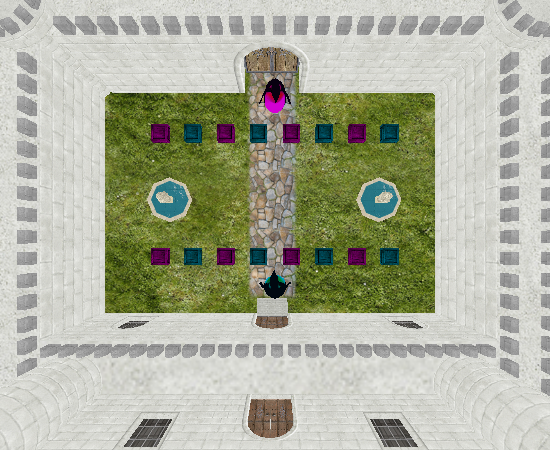
\includegraphics[scale=0.7]{images/game.png}
	\caption{Egy felülnézetes kép a játékból}
	\label{fig:game}
\end{figure}

\Section{Az elemek vezérlése}

\SubSection{Billentyű, egér funkciók}

Az ágens irányításához (lépés előre, hátra, fordulás, ugrás, doboz megfogása) különböző billenytűket haszbnáltam (például w,s,a,d) és a space-t billentyűket használtam fel, a  programból való kilépéshez az „ESC” billentyűt. Továbbá ez egér lehetővé teszi, hogy más szögből lássuk a jelenetet.

A következő függvények kerültek felhasználásra.
\begin{itemize}
\item A \texttt{glutKeyBoardFunc()}-nek három paramétere van: \texttt{key} a generált ASCII karakter, az \texttt{x} és \texttt{y} pedig az egér pozíciója abban az időpontban, mikor a billentyű lenyomás történt a \texttt{GLUT} ablakhoz képest.

Ezzel a funkcióval csak a kilépéshez szükséges \texttt{ESC} billentyű lenyomás kezelődött le és a \texttt{space}, a nyíl billentyűkhöz egy másik funkció szükséges \cite{keyboardfunc}.
\item A \texttt{glutSpecialFunc()} szükséges speciális billentyűk lenyomásának kezeléséhez,  
aminek szintén három paramétere van, a key, ami egy \texttt{GLUT\_KEY\_*} konstans, és az \texttt{x} és \texttt{y}, amik ugyanazt jelölik, mint az előző esetben, az egér relatív helyzetét az ablakhoz képest \cite{keyboardspec}.
\item A \texttt{glutMouseFunc()} az egér billentyűinek a lenyomását a  tudjuk nyomon követni, a mozgását pedig a \texttt{glutMotionFunc()}-al vagy a \texttt{glutPassiveMotionFunc()}-al. 

A glutMotionFunc azt az eshetőséget kezelei le, amikor egy vagy több billentyű lenyomás történt és közben lett mozgatva az egér. A \texttt{glutPassiveMotionFunc()} pedig azt, amikor úgy lett mozgatva az egér, hogy nem lett lenyomva egyetlen egér gomb sem \cite{mousemot},\cite{mousefunc}.
\end{itemize}

\Chapter{Interakció és kommunikáció a virtuális térben}

Ahhoz, hogy a kliensek kooperálni tudjanak a virtuális térben meg kell oldani az eszközök közötti kommunikációt.
Feltételezhetjük, hogy az eddigiekben bemutatott alkalmazásnak (továbbiakban kliensnek) van hozzáférése a helyi hálózathoz.
Ezáltal szerver-kliens architektúra szerint megoldható az eszközök közötti kommunikáció.

A következő szakaszokban azt vizsgáljuk meg, hogy a központi szerver milyen feladatokat lát ez, azzal a kommunikáció hogyan oldható meg interfészek, protokollok szintjén.

Az ezt követő részben a korábban bemutatott kliens alkalmazás kiegészítése kerül részletezésre, hogy az alkalmas legyen arra, hogy a többi klienssel megossza az adatokat a központi szerveren keresztül.

\Section{Központi szerver}

Egyenrangú kliens alkalmazásokat feltételezve a virtuális térben lévő ágensek és entitások adatait a központi szervernek kell kezelnie.
A szerverben tehát megjelenik a kliensben korábban bemutatott világmodell egy része.

Az adatmegosztási probléma tulajdonképpen úgy is tekinthető, hogy a kliensek szinkronizálják a szerverben lévő adatmodellt.
A szinkronizálásnak itt két fő iránya van.
\begin{itemize}
	\item A kliensnek le kell tudni kérdezni, hogy aktuálisan a térben hol vannak az entitások.
	\item A saját pozícióját vissza kell tudnia küldeni a szervernek.
\end{itemize}
Az elemek azonosításához szükséges, hogy minden ágensnek egyedi azonosítója legyen.

További tényező, hogy a játéknak a kezdetekor tudni kell, hogy mennyi ágens lesz majd, mivel az szerepet játszik a további elemek létrehozásában és elhelyezésében.
Egyszerűbb esetben azt mondhatjuk, hogy a szerver indításakor megadjuk, hogy mennyi ágens szerepeljen az adott térképen, majd akkor fog ténylegesen létrejönni a kooperációs tér, amikor az adott számú résztvevő már bejelentkezett.
Ezt valamilyen formában jelezni kell a kliensek felé is.
Egy lehetséges megoldás, hogy a virtuális tér állapotára vonatkozóan ilyen esetben egy speciális üzenetet kap, amelyben egyúttal az is szerepel, hogy mennyi ágens van már bejelentkezve és összesen mennyire van szükség.

% TODO: Tulajdonképpen a World adatszerkezetet kell megosztania.

% TODO: Feltételezzük, hogy egyetlen közös virtuális tér van.

\Section{REST API}

A REST alapvetően egy állapotmentes protokoll.
Az a fő előnye, hogy az erőforrások felé intézett kérésekben minden olyan információ szerepel, amely a válasz kiszámításához/összerakásához szükséges.

Tegyük fel, hogy a kooperációs teret egy \texttt{world} nevű elérési pont jelöli.
Az elérési útvonalban ezt érdemes úgy szerepeltetni, hogy \texttt{/api/world}.

\SubSection{Bejelentkezés a virtuális térbe}

\texttt{/api/login}
Egy példa kérés a szerver felé.
\begin{python}
{ "name": "Agent Name" }
\end{python}
Erre a szerver (sikeres bejelentkezés esetén) az ágens saját, egyedi azonosítójával tér vissza.
Például, hogy ha az első bejelentkező ágensről van szó, akkor
\begin{python}
{ "agent_id": 1 }
\end{python}

% TODO: Készíteni példát hibaüzenetre!

\SubSection{Entitások adatainak lekérdezése}

Az adatok lekérdezéséhez a kliens egy GET kérést küld a \texttt{world} erőforrás felé.
Az a válaszüzenetben visszaadja az összes entitás állapotát.

Tegyük fel, hogy a térben két ágens és két mozgatható elem van már csak.

% TODO: Üres üzenetre, további bejelentkezőkre váró üzenet.

\SubSection{Saját pozíció visszaküldése}

Az irányított ágens adatainak küldéséhez a klienseknek egy POST kérést kell intéznie a szerver felé.
Definiáljunk egy \texttt{agent} nevű erőforrást ehhez.
A kérésből egyértelműen ki kell derülnie, hogy az melyik ágensre vonatkozik.
Erre egy kézenfekvő megoldás, hogy ha magában az üzenetben szerepel az ágens egyedi azonosítója is, amelyet az ágens a virtuális térbe való bejelentkezéskor kap a szervertől.

% TODO: POST -> Saját pozíció felterjesztése, az ágens adatait kell szerializálni.

\begin{python}
{
  "agent_id": 1,
  "x": 10, "y": 20, "z": 30,
  "rotation": 40
}
\end{python}

\Section{Kliens alkalmazás}

A kliens alkalmazásnak a központi szerver erőforrásaihoz kell hozzáférnie.
Ilyen jellegű alkalmazásoknál tipikusan a kliens az egy webböngésző, jelen esetben viszont egy grafikus Python alkalmazásról van szó.
A kérések kezelését ilyen esetben például a \texttt{requests} modul segítségével lehet egyszerűen megoldani.

% https://www.w3schools.com/python/module_requests.asp

Feltételezhetjük, hogy a szerver szintén az alhálózaton van, továbbá, hogy az üzenetek nem túl nagy méretűek, így a kérések küldése és feldolgozása szinkron módon történhet.

\SubSection{Pozíciók interpolálása}

A rendszer szempontjából a központi szerveres megvalósítás szűk keresztmetszetet jelenthet, olyan tekintetben, hogy nem reális, hogy minden kliens minden képkocka kirajzolás előtt lekérdezi a szerveren lévő aktuális adatokat.
Tegyük fel ugyanis, hogy minden kliens 25 képkockát rajzoltat ki, és egyidejűleg 10 kliensünk van.
Hogy ha minden kliens egyszer lekérdezi az aktuális állapotot, és átküldi a saját adatait, akkor az azt jelenti, hogy másodpercenként 500 kérést kellene feldolgoznia a szervernek.
A feladat jellegéből adódik, hogy az ágensek számával a kérések száma lineárisan fog változni.
A konstans tényezőn (tehát a szükséges lekérdezések számán kliensenként) viszont lehet javítani azzal, hogy ha például a szinkronizációs pontok alacsonyabb frekvenciára vannak beállítva.
Ennek az optimális értéke függ a kliensek számától, a hálózati kommunikáció sebességétől, továbbá a szerver saját válaszidejétől.

\Section{Megbízhatóság és biztonság}

Mivel az alkalmazás több számítógépen működik egyidejűleg, ahol a kliens egy eseményvezérelt program, így több tekintetben is egy aszinkron alkalmazásról beszélhetünk.

% TODO: Szinkronizációs problémák. Mindegyik kliens egy kicsit mást lát a térből idő tekintetében is.

% TODO: Bejelentkezés, üzenetek validálása (Hasonlóan, mint bármilyen más webalkalmazás esetében) Authentikáció

% TODO: Leírni, hogy ha szinkron esetről van szó, és kiesik a szerver, akkor az összes kliens le fog fagyni, ahogy a szerver felé indít egy aktuális kérést.

\Chapter{Az elkészített alkalmazások áttekintése}

\Section{Demó programok}

Az egyes funkciók fejlesztéséhez és teszteléséhez külön kisebb programok készültek.

\begin{itemize}
	\item aruco\_test:
	A \textbf{test\_aruco.py} fájlt kell futattni.
	Az ArUco maker detektálására készítette program kód teszje. 
	
	Az images mappában szerepel 12 kép, azokon próbálja felismerni a markert, ha sikerül kirajzolja a közzépponthoz
	tartozó triédert és visszaadja a marker eltolását és elforgatását kamerához képest. (rvec, tvec)
	Az eredmény ( a kép és az adatok) a result mappába kerülnek.
	\item camera\_background\_with\_obj :
	A \textbf{camera\_cap\_with\_obj.py} fájlt kell futattni.
	A kamera képből textúra készül, majd beállítódik háttérnek és kirajzolódik rá egy objektum.
	
	Az obj objektum és mtl textúra betöltése az objloader.py-jal történik.
	A pingin modell a models mappában található.
	Kilépés 'q'-val történik.
	\item camera\_calibration :
	A \textbf{calibration.py} fájlt kell futattni.
	A kamera kalibrációja OpenCV és sakktábla minta használatával.
	A kalibrációhoz felhasznált képek az Images mappában találhatók.
	
	Az eredmény a log.json-ben tárolódik.
	Ebbe az álományba mentődik ki a kamera mátrix és a disztorziós együtthatók.
	
	A harmadik fejezetben említett kalibrációs kód, a forrásban szereplő kódot használtam fel hozzá. 
	
	Forrás: 
	
	\texttt{https://medium.com/@aliyasineser/}
	
	\texttt{opencv-camera-calibration-e9a48bdd1844}
	\item camera\_calibration\_and\_aruco\_demo:
	A \textbf{calibration.py} fájlt kell futattni.
	A harmadik fejezetben említett demó, a forrásban szereplő kódot használtam fel hozzá. 
	
	Forrás: 
	
	\texttt{https://medium.com/@aliyasineser/}
	
	\texttt{aruco-marker-tracking-with-opencv-8cb844c26628}
	\item camera\_func:
	A \textbf{camera.py} fájlt kell futattni.
	Az aktuális kameraképet visszaadó funkció szerepel benne. 
	\item camera\_texture\_on\_a\_cube:
	A \textbf{cam\_cap\_texture\_on\_cube.py} fájlt kell futattni.
	A kamera képből készült textúra kerül egy kirajzolt kockára.
	\item draw\_cube:
	A \textbf{draw\_cube.py} fájlt kell futattni.
	Egy színes oldalapokkal rendelkező kocka rajzolódik ki egy GLUT ablakba.
	\item draw\_scene:
	A \textbf{draw\_scene.py} fájlt kell futattni.
	A játék egy lehetséges kezdő állását bemutató rövid programkód.
	(Végül nem így néz ki.)
	\item draw\_texture\_from\_camera:
	A \textbf{camera\_cap\_texture.py} fájlt kell futattni.:
	Az aktuális pillanatnyi kamera képből textúra készül és ez a 
	textúra a beállítódik egy GLUT ablak háttereként. 
	\item draw\_trieder:
	A \textbf{draw\_trieder.py} fájlt kell futattni.
	A (0,0,0) pontba kirajzolódik egy triéder.
	\item game:
	A \textbf{game.py} fájlt kell futattni.
	Az elkészült program egy egyszerűbb verziója. Nem használ aruco marker felismerést, nincs szerver-kliens kommunikáció.
	Egy egyszerű OpenGL játék, amiben ugyan az a feladat, mint az elkészült programban, beletolni a dobozokat a kutakba, minden pingvin csak a saját színével megegyező dobozt tolhatja.
	Itt minden kút aktív és nincs korlátozás az egymás után egy színű dobozok eltűntetésével kapcsolatban.
	Az egyik pingvin a \texttt{w,s,a,d,e,space} a másik a \texttt{i,k,l,j,o,p} billentyűkkel irányítható.
	\item game\_with\_aruco:
	A \textbf{game.py} fájlt kell futattni.
	Az elkészült program egy próbaverziója. Itt már megtörténik a marker felismerés és az arra való rajzolás, azonban ez sem többfelhasználós.
	A szabályok ugyanazok, mint az elkészült programban, tehát minden pingvin csak a saját színével megegyező dobozt tolhatja, egyszerre csak egy kút aktív és
	pontosan annyi doboz kell bele amennyi játékos van.
	Az egyik pingvin a \texttt{w,s,a,d,e,space} a másik a \texttt{i,k,l,j,o,p} billentyűkkel irányítható.
	\item keyboard:
	A \textbf{keyboard.py} fájlt kell futattni.
	A (0,0,0) pontba kirajzolódik egy triéder. A nyíl billyentyűkkel előre, hátra illeve 
	két oldalra lehet mozogni.
	A space megnyomása után felfelé mozdul el a kamera.
	\item keyboard\_with\_cube:
	A \textbf{keyboard\_cube.py} fájlt kell futattni.
	A (0,0,0) pontba kirajzolódik egy triéder és egy kocka. A nyíl billyentyűkkel előre, hátra illeve két oldalra lehet mozogni.
	A space megnyomása után felfelé mozdul el a kocka.
	\item keyboard\_with\_obj:
	A \textbf{keyboard\_obj.py} fájlt kell futattni.
	A (0,0,0) pontba kirajzolódik egy triéder és betöltödik a pingvin modell.
	
	A nyíl billyentyűkkel előre, hátra illeve  két oldalra lehet mozogni.
	A space megnyomása után felfelé mozdul el.
	\item load\_grab\_animation:
	A \textbf{grab.py} fájlt kell futattni.
	Betöltődnek a models mappában található pingvin modellek és kirajzolódnak váltva egymást a mozulatok
	világos kék háttére. Van a mozdulatok között egy kis késeltetés.
	Az animáció a doboz tolásához a kéz emelése.
	\item load\_jump\_animation:
	A \textbf{jump.py} fájlt kell futattni.
	Betöltődnek a models mappában található pingvin modellek és kirajzolódnak váltva egymást a mozulatok
	világos kék háttére. Van a mozdulatok között egy kis késeltetés. 
	Az animáció az ugrás.
	\item load\_obj:
	A \textbf{load\_obj.py} fájlt kell futattni.
	Betöltődik a models mappában található pingvin modell és kirajzolódik egy
	világos kék háttére.
	\item load\_release\_animation:
	A \textbf{release.py} fájlt kell futattni.
	Betöltődnek a models mappában található pingvin modellek és kirajzolódnak váltva egymást a mozulatok
	világos kék háttére.
	
	Van a mozdulatok között egy kis késeltetés.
	Az animáció a doboz tolása utána a doboz elengedése.
	\item load\_walk\_animation:
	A \textbf{walk.py} fájlt kell futattni.
	Betöltődnek a models mappában található pingvin modellek és kirajzolódnak váltva egymást a mozulatok
	világos kék háttére. Van a mozdulatok között egy kis késeltetés. 
	Az animáció a sétálás.
	\item makeGlutWindow:
	A \textbf{glutwindow.py} fájlt kell futattni.
	Üres GLUT ablak nyitása, glutMainLoop használata.
	\item simple\_camera:
	A \textbf{camera.py} fájlt kell futattni.
	A kamera kép lekérése és megjelenítése OpenCV segítségével.
	Kilépés 'q'-val történik.
	\item trackAruco:
	A \textbf{trackAruco.py} fájlt kell futattni.
	A kamera kalibrációja során megkapott mátrixot és együtthatókat betöltve és
	felhasználva marker detektálás egy kapott képen.
	Ha talál markert vissza adja a marker eltolását és elforgatását kamerához képest. (rvec, tvec)
	\item trackAruco\_and\_draw\_Castle:
	A \textbf{track\_and\_draw.py} fájlt kell futattni.
	Aruco marker felismerés majd egy kastély modell rajzolása a markerre.
	\item trackAruco\_and\_draw\_Cube:
	A \textbf{track\_and\_draw.py} fájlt kell futattni.
	Aruco marker felismerés majd egy kocka rajzolása a markerre.
	\item trackAruco\_and\_draw\_model:
	A \textbf{track\_and\_draw.py} fájlt kell futattni.
	Aruco marker felismerés majd egy pingvin modell rajzolása a markerre.
\end{itemize}


A demókhoz és a programhoz felhasznált források, kódok:

\begin{itemize}
\item \texttt{https://rdmilligan.wordpress.com/2015/10/15/}

\texttt{augmented-reality-using-opencv-opengl-and-blender/}

\item \texttt{http://openglsamples.sourceforge.net/cube\_py.html }

\item \texttt{https://stackoverflow.com/questions/50764623/}


\texttt{object-is-wrong-displaced-in-ar-aruco-opengl}

\item \texttt{ https://realpython.com/python-timer/}

\item  Az objektum betöltések mindig ezzel történtek:

\texttt{https://www.pygame.org/wiki/OBJFileLoader}


\Section{A kollaborációs környezetet megvalósító program}


Felhasználható marker: 
\begin{figure}[htp]
	\centering
	
\includegraphics[scale=0.4]{images/marker.png}
	\caption{marker (forrás:https://chev.me/arucogen/)}
	\label{fig:marker}
\end{figure}


\begin{itemize}
	\item \textbf{program} (a végső program): 
	\begin{itemize}
		\item \textbf{Játékleírás}: A játék célja a dobozok eltüntetése, a szökőkutakba kell bele tolni őket.
		Minden pingvin csak a saját színével megegyező dobozt tolhatja, egyszerre csak egy kút aktív és
		pontosan annyi doboz kell bele amennyi játékos van. Ha megfelelő számú doboz kerül bele, az eddig nem aktív kút lesz az aktív.
		Ha minden doboz eltűnik, akkor ér véget a játék,nyernek a játékosok.  
		Minden játékoshoz 4 doboz tartozik, maximum négy fő vehet részt a játékban.
		\begin{figure}[htp]
			\centering
			
\includegraphics[scale=0.1]{images/win.jpg}
			\caption{A játék vége(forrás:https://miro.medium.com/max/500/1\*KOj47lkJHi9w8bxAvFAvEg.jpeg)}
			\label{fig:win}
		\end{figure}
		\item \textbf{Tesztelési lehetőség}: el kell indítani a server.py-t, aztán pedig a game.py-t, ez egyetlen kliens-t szimulál.
		Ha nem állítódik le a server.py, de a game.py újraindítódik, akkor az már a következő kliensek számít.
		A játék jelenleg 3 klienssel működik (a modellek betöltési ideje miatt), de ezt lehet bővíteni a kezdőadatok megadásával.
	\end{itemize}
	

\Chapter{Összefoglalás}


\clearpage

\addcontentsline{toc}{chapter}{Irodalomjegyzék}
\bibliographystyle{plain}
\bibliography{dolgozat.bib}

\newpage

\pagestyle{empty}

\noindent \textbf{\Large A CD melléklet tartalma}

\vskip 1cm

\noindent A dolgozathoz tartozó melléklet a következőket tartalmazza.

\begin{itemize}
\item \texttt{dolgozat.pdf}: a dolgozat PDF fájl formájában,
\item \texttt{szakdolgozat}: a dolgozat \LaTeX\ forráskódját tartalmazó jegyzék,
\item \texttt{programok}: az elkészített programokat tartalmazó jegyzék.
\end{itemize}

\bigskip

A programok teszteléséhez a következő hardver és szoftver eszközökre van szükség.
\begin{itemize}
	\item Kamera,
	\item egy, a megfelelő könyvtárba tartozó ArUco marker,
	\item \textit{OpenCV} és \textit{ArUco} függvénykönyvtárak a kamerapozíció becsléséhez,
	\item \textit{PyOpenGL} és \textit{PyGame} függvénykönyvtárak a megjelenítéshez,
	\item \texttt{falcon}, \texttt{waitress} és \texttt{requests} csomagok a szerver és kliens közötti kommunikációhoz.
\end{itemize}




\end{document}
